\documentclass[a4paper]{book}
\usepackage{makeidx}
\usepackage{natbib}
\usepackage{graphicx}
\usepackage{multicol}
\usepackage{float}
\usepackage{listings}
\usepackage{color}
\usepackage{ifthen}
\usepackage[table]{xcolor}
\usepackage{textcomp}
\usepackage{alltt}
\usepackage{ifpdf}
\ifpdf
\usepackage[pdftex,
            pagebackref=true,
            colorlinks=true,
            linkcolor=blue,
            unicode
           ]{hyperref}
\else
\usepackage[ps2pdf,
            pagebackref=true,
            colorlinks=true,
            linkcolor=blue,
            unicode
           ]{hyperref}
\usepackage{pspicture}
\fi
\usepackage[utf8]{inputenc}
\usepackage{mathptmx}
\usepackage[scaled=.90]{helvet}
\usepackage{courier}
\usepackage{sectsty}
\usepackage[titles]{tocloft}
\usepackage{doxygen}
\lstset{language=C++,inputencoding=utf8,basicstyle=\footnotesize,breaklines=true,breakatwhitespace=true,tabsize=8,numbers=left }
\makeindex
\setcounter{tocdepth}{3}
\renewcommand{\footrulewidth}{0.4pt}
\renewcommand{\familydefault}{\sfdefault}
\hfuzz=15pt
\setlength{\emergencystretch}{15pt}
\hbadness=750
\tolerance=750
\begin{document}
\hypersetup{pageanchor=false,citecolor=blue}
\begin{titlepage}
\vspace*{7cm}
\begin{center}
{\Large \-S\-S\-N }\\
\vspace*{1cm}
{\large \-Generated by Doxygen 1.7.6.1}\\
\vspace*{0.5cm}
{\small Thu Apr 5 2012 13:26:35}\\
\end{center}
\end{titlepage}
\clearemptydoublepage
\pagenumbering{roman}
\tableofcontents
\clearemptydoublepage
\pagenumbering{arabic}
\hypersetup{pageanchor=true,citecolor=blue}
\chapter{\-Class \-Index}
\section{\-Class \-Hierarchy}
\-This inheritance list is sorted roughly, but not completely, alphabetically\-:\begin{DoxyCompactList}
\item \contentsline{section}{\-Activation\-Function$<$ \-T $>$}{\pageref{class_activation_function}}{}
\item \contentsline{section}{\-Helper}{\pageref{class_helper}}{}
\item \contentsline{section}{\-Input$<$ \-T $>$}{\pageref{class_input}}{}
\begin{DoxyCompactList}
\item \contentsline{section}{\-Bias$<$ \-T $>$}{\pageref{class_bias}}{}
\item \contentsline{section}{\-Entry$<$ \-T $>$}{\pageref{class_entry}}{}
\item \contentsline{section}{\-Neuron$<$ \-T, \-Activation\-Function $>$}{\pageref{class_neuron}}{}
\end{DoxyCompactList}
\item \contentsline{section}{\-Linear\-Activation\-Function$<$ \-T $>$}{\pageref{class_linear_activation_function}}{}
\item \contentsline{section}{\-Link$<$ \-T $>$}{\pageref{class_link}}{}
\item \contentsline{section}{\-Neural\-Network$<$ \-T, \-Activation\-Function $>$}{\pageref{class_neural_network}}{}
\item \contentsline{section}{\-Output$<$ \-T $>$}{\pageref{class_output}}{}
\begin{DoxyCompactList}
\item \contentsline{section}{\-Exit$<$ \-T $>$}{\pageref{class_exit}}{}
\item \contentsline{section}{\-Neuron$<$ \-T, \-Activation\-Function $>$}{\pageref{class_neuron}}{}
\end{DoxyCompactList}
\item \contentsline{section}{\-Step\-Activation\-Function$<$ \-T $>$}{\pageref{class_step_activation_function}}{}
\item \contentsline{section}{\-Neural\-Network$<$ \-T, \-Activation\-Function $>$\-:\-:\-Wrong\-Argument}{\pageref{class_neural_network_1_1_wrong_argument}}{}
\item \contentsline{section}{\-Neural\-Network$<$ \-T, \-Activation\-Function $>$\-:\-:\-Wrong\-State}{\pageref{class_neural_network_1_1_wrong_state}}{}
\end{DoxyCompactList}

\chapter{\-Class \-Index}
\section{\-Class \-List}
\-Here are the classes, structs, unions and interfaces with brief descriptions\-:\begin{DoxyCompactList}
\item\contentsline{section}{\hyperlink{class_activation_function}{\-Activation\-Function$<$ T $>$} }{\pageref{class_activation_function}}{}
\item\contentsline{section}{\hyperlink{class_bias}{\-Bias$<$ T $>$} }{\pageref{class_bias}}{}
\item\contentsline{section}{\hyperlink{class_entry}{\-Entry$<$ T $>$} }{\pageref{class_entry}}{}
\item\contentsline{section}{\hyperlink{class_exit}{\-Exit$<$ T $>$} }{\pageref{class_exit}}{}
\item\contentsline{section}{\hyperlink{class_helper}{\-Helper} }{\pageref{class_helper}}{}
\item\contentsline{section}{\hyperlink{class_input}{\-Input$<$ T $>$} }{\pageref{class_input}}{}
\item\contentsline{section}{\hyperlink{class_linear_activation_function}{\-Linear\-Activation\-Function$<$ T $>$} }{\pageref{class_linear_activation_function}}{}
\item\contentsline{section}{\hyperlink{class_link}{\-Link$<$ T $>$} }{\pageref{class_link}}{}
\item\contentsline{section}{\hyperlink{class_neural_network}{\-Neural\-Network$<$ T, Activation\-Function $>$} }{\pageref{class_neural_network}}{}
\item\contentsline{section}{\hyperlink{class_neuron}{\-Neuron$<$ T, Activation\-Function $>$} }{\pageref{class_neuron}}{}
\item\contentsline{section}{\hyperlink{class_output}{\-Output$<$ T $>$} }{\pageref{class_output}}{}
\item\contentsline{section}{\hyperlink{class_step_activation_function}{\-Step\-Activation\-Function$<$ T $>$} }{\pageref{class_step_activation_function}}{}
\item\contentsline{section}{\hyperlink{class_neural_network_1_1_wrong_argument}{\-Neural\-Network$<$ T, Activation\-Function $>$\-::\-Wrong\-Argument} }{\pageref{class_neural_network_1_1_wrong_argument}}{}
\item\contentsline{section}{\hyperlink{class_neural_network_1_1_wrong_state}{\-Neural\-Network$<$ T, Activation\-Function $>$\-::\-Wrong\-State} }{\pageref{class_neural_network_1_1_wrong_state}}{}
\end{DoxyCompactList}

\chapter{\-Class \-Documentation}
\hypertarget{class_activation_function}{\section{\-Activation\-Function$<$ \-T $>$ \-Class \-Template \-Reference}
\label{class_activation_function}\index{\-Activation\-Function$<$ T $>$@{\-Activation\-Function$<$ T $>$}}
}
\subsection*{\-Public \-Member \-Functions}
\begin{DoxyCompactItemize}
\item 
\-T \hyperlink{class_activation_function_a34df0907340f36e41d5a1fd60a015036}{operator()} (\-T x) const =0
\item 
\-T \hyperlink{class_activation_function_a6916cffe74a85a7737b032e8977d3192}{deriterative} (\-T x) const =0
\end{DoxyCompactItemize}
\subsubsection*{template$<$class T$>$ class Activation\-Function$<$ T $>$}



\subsection{\-Member \-Function \-Documentation}
\hypertarget{class_activation_function_a6916cffe74a85a7737b032e8977d3192}{\index{\-Activation\-Function@{\-Activation\-Function}!deriterative@{deriterative}}
\index{deriterative@{deriterative}!ActivationFunction@{\-Activation\-Function}}
\subsubsection[{deriterative}]{\setlength{\rightskip}{0pt plus 5cm}template$<$class T $>$ \-T {\bf \-Activation\-Function}$<$ \-T $>$\-::{\bf deriterative} (
\begin{DoxyParamCaption}
\item[{\-T}]{x}
\end{DoxyParamCaption}
) const\hspace{0.3cm}{\ttfamily  \mbox{[}pure virtual\mbox{]}}}}\label{class_activation_function_a6916cffe74a85a7737b032e8977d3192}
\-Funkcja licząca pochodną funkcji skokowej (jako cos(x) w zakresie 0 do 1) 
\begin{DoxyParams}{\-Parameters}
{\em x} & \\
\hline
\end{DoxyParams}
\begin{DoxyReturn}{\-Returns}

\end{DoxyReturn}
\hypertarget{class_activation_function_a34df0907340f36e41d5a1fd60a015036}{\index{\-Activation\-Function@{\-Activation\-Function}!operator()@{operator()}}
\index{operator()@{operator()}!ActivationFunction@{\-Activation\-Function}}
\subsubsection[{operator()}]{\setlength{\rightskip}{0pt plus 5cm}template$<$class T $>$ \-T {\bf \-Activation\-Function}$<$ \-T $>$\-::operator() (
\begin{DoxyParamCaption}
\item[{\-T}]{x}
\end{DoxyParamCaption}
) const\hspace{0.3cm}{\ttfamily  \mbox{[}pure virtual\mbox{]}}}}\label{class_activation_function_a34df0907340f36e41d5a1fd60a015036}
\-Funkcja sprawdzająca czy dana wartość jest większa od podanego progu. 
\begin{DoxyParams}{\-Parameters}
{\em x} & \-Sprawdzana wartość. \\
\hline
\end{DoxyParams}
\begin{DoxyReturn}{\-Returns}
true jeśli sprawdzana waratość jest większa, false w przeciwnym wypadku. 
\end{DoxyReturn}


\-The documentation for this class was generated from the following file\-:\begin{DoxyCompactItemize}
\item 
/home/tomko/moje\-\_\-dziela/\-S\-S\-N/\-Neuron/\-Activation\-Function.\-h\end{DoxyCompactItemize}

\hypertarget{class_bias}{\section{\-Bias$<$ \-T $>$ \-Class \-Template \-Reference}
\label{class_bias}\index{\-Bias$<$ T $>$@{\-Bias$<$ T $>$}}
}


{\ttfamily \#include $<$\-Bias.\-h$>$}

\-Inheritance diagram for \-Bias$<$ \-T $>$\-:\begin{figure}[H]
\begin{center}
\leavevmode
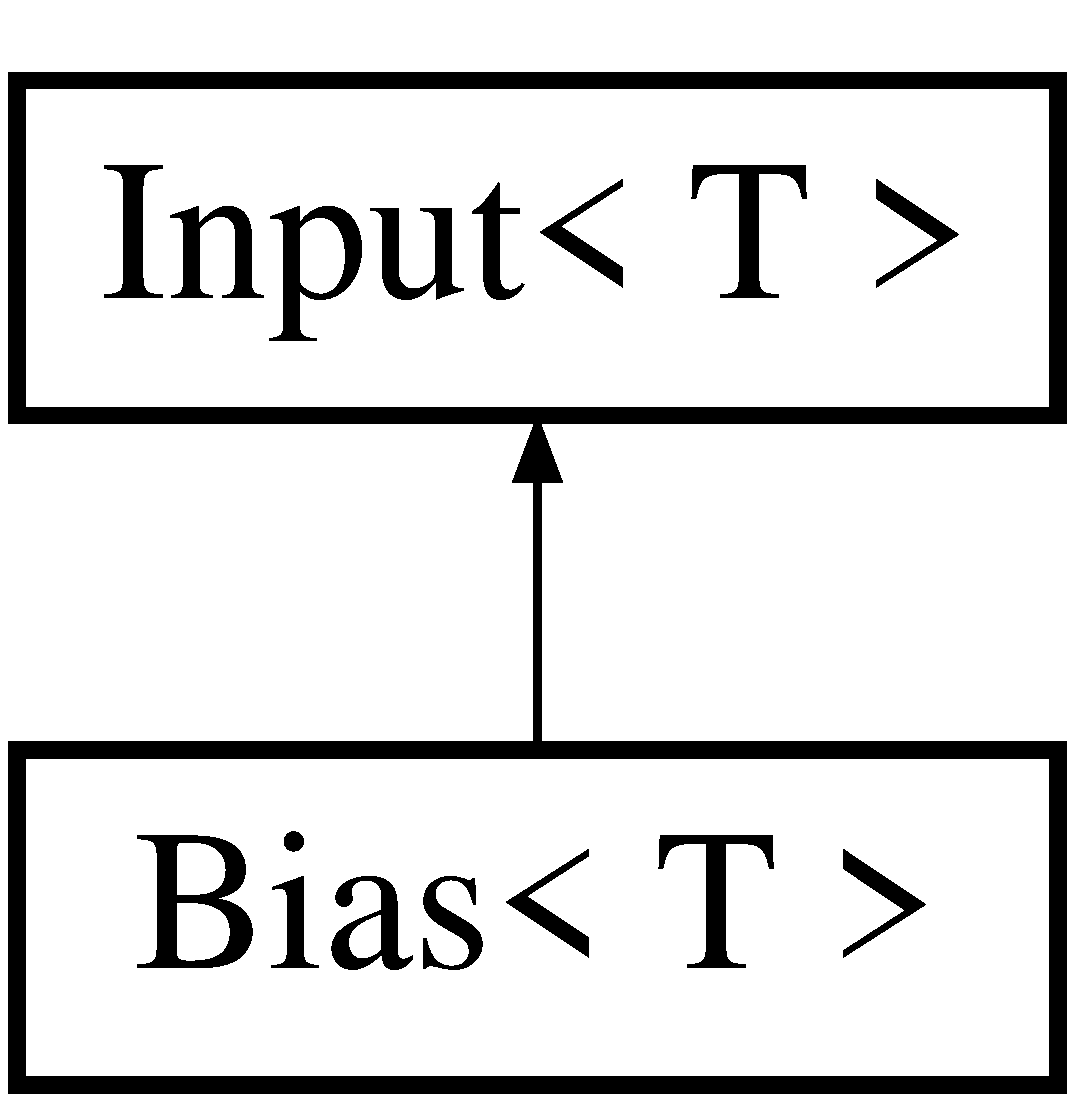
\includegraphics[height=2.000000cm]{class_bias}
\end{center}
\end{figure}
\subsection*{\-Public \-Member \-Functions}
\begin{DoxyCompactItemize}
\item 
\hyperlink{class_bias_abb349bc7ef3317db4a7ce75c96dbb533}{\-Bias} (\-T i)
\item 
void \hyperlink{class_bias_ab6df47ae8047f915cfa1fb77683b0eb7}{set\-Bias} (\-T i)
\item 
void \hyperlink{class_bias_a5489ed8d5ecb5bd14e21532968bb3027}{set\-Bias\-And\-Send} (\-T i)
\item 
void \hyperlink{class_bias_a3bf2cdb0a52508399df31b9f7dcf358b}{send\-Bias\-To\-Links} ()
\end{DoxyCompactItemize}


\subsection{\-Detailed \-Description}
\subsubsection*{template$<$class T$>$class Bias$<$ T $>$}

\-Odpowiada przesunięciu w sieciach neuronowych. \-Po podłączeniu linku należy przekazać wartość do łącz lub użyć metody \hyperlink{class_bias_ab6df47ae8047f915cfa1fb77683b0eb7}{set\-Bias(\-T)}. 

\subsection{\-Constructor \& \-Destructor \-Documentation}
\hypertarget{class_bias_abb349bc7ef3317db4a7ce75c96dbb533}{\index{\-Bias@{\-Bias}!\-Bias@{\-Bias}}
\index{\-Bias@{\-Bias}!Bias@{\-Bias}}
\subsubsection[{\-Bias}]{\setlength{\rightskip}{0pt plus 5cm}template$<$class T $>$ {\bf \-Bias}$<$ \-T $>$\-::{\bf \-Bias} (
\begin{DoxyParamCaption}
\item[{\-T}]{i}
\end{DoxyParamCaption}
)\hspace{0.3cm}{\ttfamily  \mbox{[}inline\mbox{]}}}}\label{class_bias_abb349bc7ef3317db4a7ce75c96dbb533}
\-Konstruktor ustawiający początkową wartość przesunięcia. \-Po podłączeniu linku należy przekazać wartość do łącz lub użyć metody \hyperlink{class_bias_ab6df47ae8047f915cfa1fb77683b0eb7}{set\-Bias(\-T)}. 
\begin{DoxyParams}{\-Parameters}
{\em i} & \-Wartość przesunięcia. \\
\hline
\end{DoxyParams}


\subsection{\-Member \-Function \-Documentation}
\hypertarget{class_bias_a3bf2cdb0a52508399df31b9f7dcf358b}{\index{\-Bias@{\-Bias}!send\-Bias\-To\-Links@{send\-Bias\-To\-Links}}
\index{send\-Bias\-To\-Links@{send\-Bias\-To\-Links}!Bias@{\-Bias}}
\subsubsection[{send\-Bias\-To\-Links}]{\setlength{\rightskip}{0pt plus 5cm}template$<$class T $>$ void {\bf \-Bias}$<$ \-T $>$\-::{\bf send\-Bias\-To\-Links} (
\begin{DoxyParamCaption}
{}
\end{DoxyParamCaption}
)\hspace{0.3cm}{\ttfamily  \mbox{[}inline\mbox{]}}}}\label{class_bias_a3bf2cdb0a52508399df31b9f7dcf358b}
\-Wysyła wartość przesunięcia do łącz. \hypertarget{class_bias_ab6df47ae8047f915cfa1fb77683b0eb7}{\index{\-Bias@{\-Bias}!set\-Bias@{set\-Bias}}
\index{set\-Bias@{set\-Bias}!Bias@{\-Bias}}
\subsubsection[{set\-Bias}]{\setlength{\rightskip}{0pt plus 5cm}template$<$class T $>$ void {\bf \-Bias}$<$ \-T $>$\-::{\bf set\-Bias} (
\begin{DoxyParamCaption}
\item[{\-T}]{i}
\end{DoxyParamCaption}
)\hspace{0.3cm}{\ttfamily  \mbox{[}inline\mbox{]}}}}\label{class_bias_ab6df47ae8047f915cfa1fb77683b0eb7}
\-Ustawia wartość przesunięcia i nie wysyła jej do łącz. 
\begin{DoxyParams}{\-Parameters}
{\em i} & \-Wartość przesunięcia. \\
\hline
\end{DoxyParams}
\hypertarget{class_bias_a5489ed8d5ecb5bd14e21532968bb3027}{\index{\-Bias@{\-Bias}!set\-Bias\-And\-Send@{set\-Bias\-And\-Send}}
\index{set\-Bias\-And\-Send@{set\-Bias\-And\-Send}!Bias@{\-Bias}}
\subsubsection[{set\-Bias\-And\-Send}]{\setlength{\rightskip}{0pt plus 5cm}template$<$class T $>$ void {\bf \-Bias}$<$ \-T $>$\-::{\bf set\-Bias\-And\-Send} (
\begin{DoxyParamCaption}
\item[{\-T}]{i}
\end{DoxyParamCaption}
)\hspace{0.3cm}{\ttfamily  \mbox{[}inline\mbox{]}}}}\label{class_bias_a5489ed8d5ecb5bd14e21532968bb3027}
\-Ustawia wartość przesunięcia i wysyła ją do łącz. 
\begin{DoxyParams}{\-Parameters}
{\em i} & \-Wartość przesunięcia. \\
\hline
\end{DoxyParams}


\-The documentation for this class was generated from the following file\-:\begin{DoxyCompactItemize}
\item 
\-Neuron/\-Bias.\-h\end{DoxyCompactItemize}

\hypertarget{class_entry}{\section{\-Entry$<$ \-T $>$ \-Class \-Template \-Reference}
\label{class_entry}\index{\-Entry$<$ T $>$@{\-Entry$<$ T $>$}}
}


{\ttfamily \#include $<$\-Entry.\-h$>$}

\-Inheritance diagram for \-Entry$<$ \-T $>$\-:\begin{figure}[H]
\begin{center}
\leavevmode
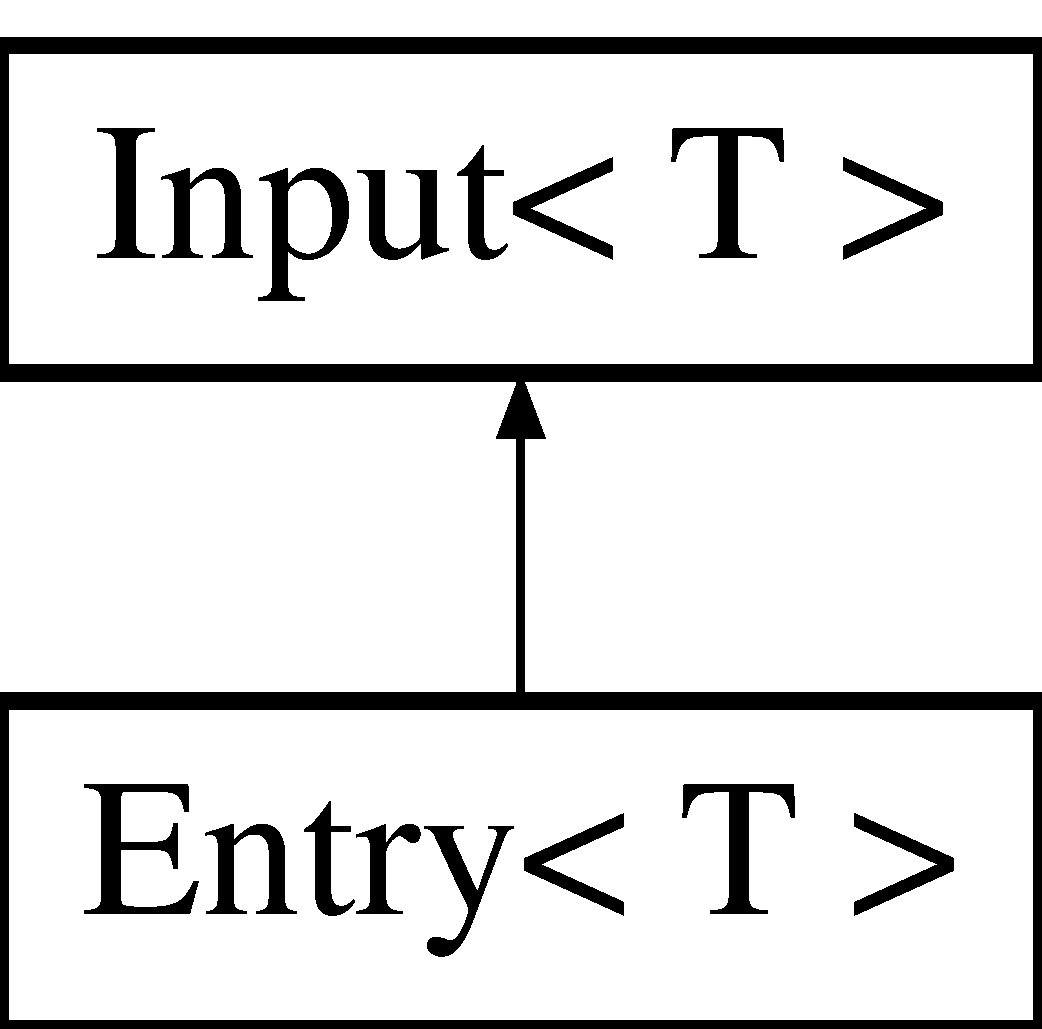
\includegraphics[height=2.000000cm]{class_entry}
\end{center}
\end{figure}
\subsection*{\-Public \-Member \-Functions}
\begin{DoxyCompactItemize}
\item 
\hypertarget{class_entry_aa5b0b7444339efa02150964d4f82e18d}{{\bfseries \-Entry} (const \hyperlink{class_entry}{\-Entry} \&orig)}\label{class_entry_aa5b0b7444339efa02150964d4f82e18d}

\item 
void \hyperlink{class_entry_afdde8cf7183ac5a343fbe993f361be4f}{set\-Entry} (\-T entry)
\end{DoxyCompactItemize}


\subsection{\-Detailed \-Description}
\subsubsection*{template$<$class T$>$class Entry$<$ T $>$}

\-Klasa \hyperlink{class_entry}{\-Entry} odpowiada wejściom do sieci neuronowej. 

\subsection{\-Member \-Function \-Documentation}
\hypertarget{class_entry_afdde8cf7183ac5a343fbe993f361be4f}{\index{\-Entry@{\-Entry}!set\-Entry@{set\-Entry}}
\index{set\-Entry@{set\-Entry}!Entry@{\-Entry}}
\subsubsection[{set\-Entry}]{\setlength{\rightskip}{0pt plus 5cm}template$<$class T $>$ void {\bf \-Entry}$<$ \-T $>$\-::{\bf set\-Entry} (
\begin{DoxyParamCaption}
\item[{\-T}]{entry}
\end{DoxyParamCaption}
)\hspace{0.3cm}{\ttfamily  \mbox{[}inline\mbox{]}}}}\label{class_entry_afdde8cf7183ac5a343fbe993f361be4f}
\-Ustawia wejście na podaną wartość. 
\begin{DoxyParams}{\-Parameters}
{\em entry} & Żądana wartość. \\
\hline
\end{DoxyParams}


\-The documentation for this class was generated from the following file\-:\begin{DoxyCompactItemize}
\item 
\-Neuron/\-Entry.\-h\end{DoxyCompactItemize}

\hypertarget{class_exit}{\section{\-Exit$<$ \-T $>$ \-Class \-Template \-Reference}
\label{class_exit}\index{\-Exit$<$ T $>$@{\-Exit$<$ T $>$}}
}


{\ttfamily \#include $<$\-Exit.\-h$>$}

\-Inheritance diagram for \-Exit$<$ \-T $>$\-:\begin{figure}[H]
\begin{center}
\leavevmode
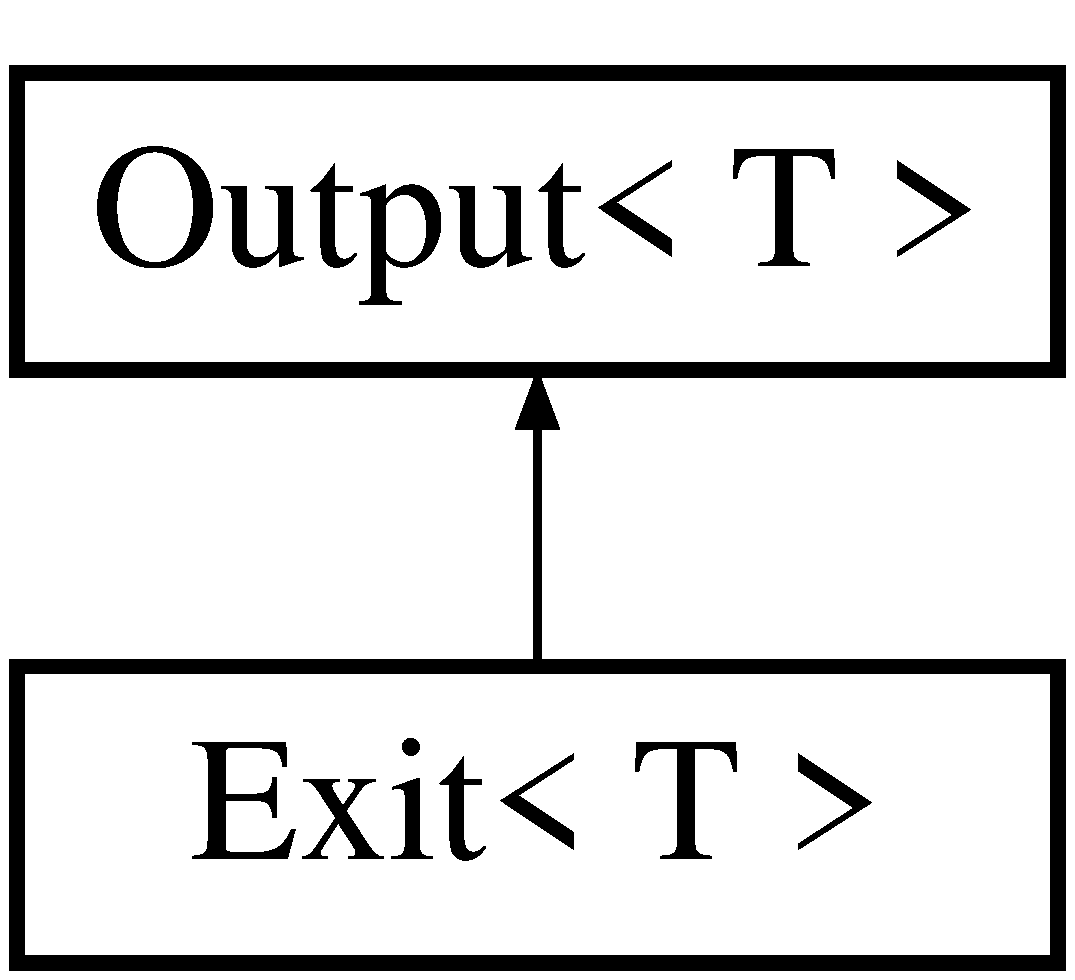
\includegraphics[height=2.000000cm]{class_exit}
\end{center}
\end{figure}
\subsection*{\-Public \-Member \-Functions}
\begin{DoxyCompactItemize}
\item 
\hypertarget{class_exit_acad725c8d30560b30b7d0e12eea95ccd}{{\bfseries \-Exit} (const \hyperlink{class_exit}{\-Exit} \&orig)}\label{class_exit_acad725c8d30560b30b7d0e12eea95ccd}

\item 
\-T \hyperlink{class_exit_ace64923bf5842a32f0abbb413e0bc50f}{get\-Exit} () const 
\item 
void \hyperlink{class_exit_a7579d52eedde1485a1f812b4edad463c}{learn} (\-T answer) const 
\end{DoxyCompactItemize}


\subsection{\-Detailed \-Description}
\subsubsection*{template$<$class T$>$class Exit$<$ T $>$}

\-Klasa \hyperlink{class_exit}{\-Exit} odpowiada wyjściom z sieci neuronowej 

\subsection{\-Member \-Function \-Documentation}
\hypertarget{class_exit_ace64923bf5842a32f0abbb413e0bc50f}{\index{\-Exit@{\-Exit}!get\-Exit@{get\-Exit}}
\index{get\-Exit@{get\-Exit}!Exit@{\-Exit}}
\subsubsection[{get\-Exit}]{\setlength{\rightskip}{0pt plus 5cm}template$<$class T $>$ \-T {\bf \-Exit}$<$ \-T $>$\-::{\bf get\-Exit} (
\begin{DoxyParamCaption}
{}
\end{DoxyParamCaption}
) const\hspace{0.3cm}{\ttfamily  \mbox{[}inline\mbox{]}}}}\label{class_exit_ace64923bf5842a32f0abbb413e0bc50f}
\-Funkcja zwracająca wyjście. \begin{DoxyReturn}{\-Returns}
\-Wyjście. 
\end{DoxyReturn}
\hypertarget{class_exit_a7579d52eedde1485a1f812b4edad463c}{\index{\-Exit@{\-Exit}!learn@{learn}}
\index{learn@{learn}!Exit@{\-Exit}}
\subsubsection[{learn}]{\setlength{\rightskip}{0pt plus 5cm}template$<$class T $>$ void {\bf \-Exit}$<$ \-T $>$\-::{\bf learn} (
\begin{DoxyParamCaption}
\item[{\-T}]{answer}
\end{DoxyParamCaption}
) const\hspace{0.3cm}{\ttfamily  \mbox{[}inline\mbox{]}}}}\label{class_exit_a7579d52eedde1485a1f812b4edad463c}
\-Funkcja rozpoczynająca uczenienie z tego wyjścia sieci. 
\begin{DoxyParams}{\-Parameters}
{\em answer} & Żądana odpowiedź. \\
\hline
\end{DoxyParams}


\-The documentation for this class was generated from the following file\-:\begin{DoxyCompactItemize}
\item 
/home/tomko/moje\-\_\-dziela/\-S\-S\-N/\-Neuron/\-Exit.\-h\end{DoxyCompactItemize}

\hypertarget{class_helper}{\section{\-Helper \-Class \-Reference}
\label{class_helper}\index{\-Helper@{\-Helper}}
}
\subsection*{\-Static \-Public \-Member \-Functions}
\begin{DoxyCompactItemize}
\item 
static std\-::string \hyperlink{class_helper_aea19db1a4a7d6d3d793584fe8afab244}{int\-To\-String} (int n)
\item 
static std\-::string \hyperlink{class_helper_a43074fd7be9b2f43cc6e34941b25cc63}{double\-To\-String} (double n)
\end{DoxyCompactItemize}


\subsection{\-Member \-Function \-Documentation}
\hypertarget{class_helper_a43074fd7be9b2f43cc6e34941b25cc63}{\index{\-Helper@{\-Helper}!double\-To\-String@{double\-To\-String}}
\index{double\-To\-String@{double\-To\-String}!Helper@{\-Helper}}
\subsubsection[{double\-To\-String}]{\setlength{\rightskip}{0pt plus 5cm}string {\bf \-Helper\-::double\-To\-String} (
\begin{DoxyParamCaption}
\item[{double}]{n}
\end{DoxyParamCaption}
)\hspace{0.3cm}{\ttfamily  \mbox{[}static\mbox{]}}}}\label{class_helper_a43074fd7be9b2f43cc6e34941b25cc63}
\-Funkcja zmieniająca double na std\-::string 
\begin{DoxyParams}{\-Parameters}
{\em n} & double do zmiany. \\
\hline
\end{DoxyParams}
\begin{DoxyReturn}{\-Returns}
std\-::string odpowiadający danej liczbie. 
\end{DoxyReturn}
\hypertarget{class_helper_aea19db1a4a7d6d3d793584fe8afab244}{\index{\-Helper@{\-Helper}!int\-To\-String@{int\-To\-String}}
\index{int\-To\-String@{int\-To\-String}!Helper@{\-Helper}}
\subsubsection[{int\-To\-String}]{\setlength{\rightskip}{0pt plus 5cm}string {\bf \-Helper\-::int\-To\-String} (
\begin{DoxyParamCaption}
\item[{int}]{n}
\end{DoxyParamCaption}
)\hspace{0.3cm}{\ttfamily  \mbox{[}static\mbox{]}}}}\label{class_helper_aea19db1a4a7d6d3d793584fe8afab244}
\-Funkcja zamieniająca integer na string. 
\begin{DoxyParams}{\-Parameters}
{\em n} & \-Integer, który chcemy zamienić. \\
\hline
\end{DoxyParams}
\begin{DoxyReturn}{\-Returns}
\-String odpowiadający tej liczbie. \-Jeśli przekazana liczba nie jest całkowita to następuje obcięcie (np. z 5.\-6 tworzone jest \char`\"{}5\char`\"{}). 
\end{DoxyReturn}


\-The documentation for this class was generated from the following files\-:\begin{DoxyCompactItemize}
\item 
\-Lib\-Helper/\-Helper.\-h\item 
\-Lib\-Helper/\-Helper.\-cpp\end{DoxyCompactItemize}

\hypertarget{class_input}{\section{\-Input$<$ \-T $>$ \-Class \-Template \-Reference}
\label{class_input}\index{\-Input$<$ T $>$@{\-Input$<$ T $>$}}
}


{\ttfamily \#include $<$\-Input.\-h$>$}

\-Inheritance diagram for \-Input$<$ \-T $>$\-:\begin{figure}[H]
\begin{center}
\leavevmode
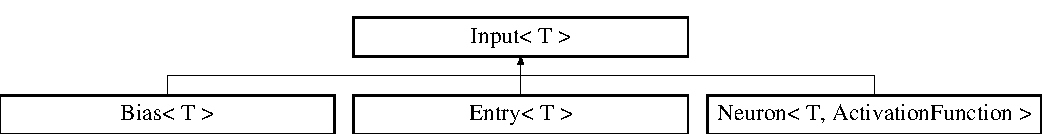
\includegraphics[height=1.803543cm]{class_input}
\end{center}
\end{figure}
\subsection*{\-Public \-Member \-Functions}
\begin{DoxyCompactItemize}
\item 
virtual \-T \hyperlink{class_input_acd4a6ffcb32722a8f7dddf37b9ed0a66}{get\-Value} () const 
\item 
void \hyperlink{class_input_a74abbc00098fc83a0d6b1c67f4590464}{set\-Link\-Out} (\hyperlink{class_link}{\-Link}$<$ \-T $>$ $\ast$link)
\end{DoxyCompactItemize}
\subsection*{\-Protected \-Member \-Functions}
\begin{DoxyCompactItemize}
\item 
void \hyperlink{class_input_afa18c71eae21a7233fd6865e44c25df0}{set\-Val\-To\-Auts} () const 
\end{DoxyCompactItemize}
\subsection*{\-Protected \-Attributes}
\begin{DoxyCompactItemize}
\item 
\hypertarget{class_input_aa2eb098d4f45d4ff4fcd2206fab7f3e5}{\-T {\bfseries input\-\_\-value}}\label{class_input_aa2eb098d4f45d4ff4fcd2206fab7f3e5}

\item 
\hypertarget{class_input_add27905b0d403f8908cf2bf7a95b740f}{std\-::list$<$ \hyperlink{class_link}{\-Link}$<$ \-T $>$ $\ast$ $>$ {\bfseries outs}}\label{class_input_add27905b0d403f8908cf2bf7a95b740f}

\end{DoxyCompactItemize}


\subsection{\-Detailed \-Description}
\subsubsection*{template$<$class \-T$>$class Input$<$ T $>$}

\-Klasa \hyperlink{class_input}{\-Input} jest interfejsem wejścia do klasy \hyperlink{class_link}{\-Link}. 

\subsection{\-Member \-Function \-Documentation}
\hypertarget{class_input_acd4a6ffcb32722a8f7dddf37b9ed0a66}{\index{\-Input@{\-Input}!get\-Value@{get\-Value}}
\index{get\-Value@{get\-Value}!Input@{\-Input}}
\subsubsection[{get\-Value}]{\setlength{\rightskip}{0pt plus 5cm}template$<$class \-T$>$ virtual \-T {\bf \-Input}$<$ \-T $>$\-::{\bf get\-Value} (
\begin{DoxyParamCaption}
{}
\end{DoxyParamCaption}
) const\hspace{0.3cm}{\ttfamily  \mbox{[}inline, virtual\mbox{]}}}}\label{class_input_acd4a6ffcb32722a8f7dddf37b9ed0a66}
\-Funkcja zwracająca przechowywaną wartość do połączeń. \begin{DoxyReturn}{\-Returns}
\-Przechowywana wartość. 
\end{DoxyReturn}
\hypertarget{class_input_a74abbc00098fc83a0d6b1c67f4590464}{\index{\-Input@{\-Input}!set\-Link\-Out@{set\-Link\-Out}}
\index{set\-Link\-Out@{set\-Link\-Out}!Input@{\-Input}}
\subsubsection[{set\-Link\-Out}]{\setlength{\rightskip}{0pt plus 5cm}template$<$class \-T$>$ void {\bf \-Input}$<$ \-T $>$\-::{\bf set\-Link\-Out} (
\begin{DoxyParamCaption}
\item[{{\bf \-Link}$<$ \-T $>$ $\ast$}]{link}
\end{DoxyParamCaption}
)\hspace{0.3cm}{\ttfamily  \mbox{[}inline\mbox{]}}}}\label{class_input_a74abbc00098fc83a0d6b1c67f4590464}
\-Funkcja dodająca połączenie do wejścia do połączenia. 
\begin{DoxyParams}{\-Parameters}
{\em link} & \-Dodawane połączenie. \\
\hline
\end{DoxyParams}
\hypertarget{class_input_afa18c71eae21a7233fd6865e44c25df0}{\index{\-Input@{\-Input}!set\-Val\-To\-Auts@{set\-Val\-To\-Auts}}
\index{set\-Val\-To\-Auts@{set\-Val\-To\-Auts}!Input@{\-Input}}
\subsubsection[{set\-Val\-To\-Auts}]{\setlength{\rightskip}{0pt plus 5cm}template$<$class \-T$>$ void {\bf \-Input}$<$ \-T $>$\-::{\bf set\-Val\-To\-Auts} (
\begin{DoxyParamCaption}
{}
\end{DoxyParamCaption}
) const\hspace{0.3cm}{\ttfamily  \mbox{[}inline, protected\mbox{]}}}}\label{class_input_afa18c71eae21a7233fd6865e44c25df0}
\-Wysłanie wartości przechowywanej w danym obiekcie do wszystkich podłączonych linków. 

\-The documentation for this class was generated from the following file\-:\begin{DoxyCompactItemize}
\item 
/home/tomko/moje\-\_\-dziela/\-S\-S\-N/\-Neuron/\-Input.\-h\end{DoxyCompactItemize}

\hypertarget{class_linear_activation_function}{\section{\-Linear\-Activation\-Function$<$ \-T $>$ \-Class \-Template \-Reference}
\label{class_linear_activation_function}\index{\-Linear\-Activation\-Function$<$ T $>$@{\-Linear\-Activation\-Function$<$ T $>$}}
}


{\ttfamily \#include $<$\-Linear\-Activation\-Function.\-h$>$}

\subsection*{\-Public \-Member \-Functions}
\begin{DoxyCompactItemize}
\item 
\hyperlink{class_linear_activation_function_a0474630a90119eb50d775b3e9aa46b30}{\-Linear\-Activation\-Function} ()
\item 
\hyperlink{class_linear_activation_function_ada030e1ea55f5127fdd7455279177be1}{\-Linear\-Activation\-Function} (double p)
\item 
\-T \hyperlink{class_linear_activation_function_a97e4c739f6cfb4b8b639e5921f6d4733}{operator()} (\-T x)
\item 
\hypertarget{class_linear_activation_function_aed111abd3fbc37e8a0faff788258a97d}{\-T {\bfseries deriterative} (\-T x)}\label{class_linear_activation_function_aed111abd3fbc37e8a0faff788258a97d}

\item 
void \hyperlink{class_linear_activation_function_ad7a5e2511224ce15c616e1aac7f95706}{set\-Parameter} (double parameter)
\end{DoxyCompactItemize}


\subsection{\-Detailed \-Description}
\subsubsection*{template$<$class T$>$class Linear\-Activation\-Function$<$ T $>$}

\-Klasa przedstawiającą skokową funkcję aktywacji o kształcie sigmoidy parametryzowana wartością określającą w jakim zakresie jest największa zmiana wartości. 

\subsection{\-Constructor \& \-Destructor \-Documentation}
\hypertarget{class_linear_activation_function_a0474630a90119eb50d775b3e9aa46b30}{\index{\-Linear\-Activation\-Function@{\-Linear\-Activation\-Function}!\-Linear\-Activation\-Function@{\-Linear\-Activation\-Function}}
\index{\-Linear\-Activation\-Function@{\-Linear\-Activation\-Function}!LinearActivationFunction@{\-Linear\-Activation\-Function}}
\subsubsection[{\-Linear\-Activation\-Function}]{\setlength{\rightskip}{0pt plus 5cm}template$<$class T $>$ {\bf \-Linear\-Activation\-Function}$<$ \-T $>$\-::{\bf \-Linear\-Activation\-Function} (
\begin{DoxyParamCaption}
{}
\end{DoxyParamCaption}
)\hspace{0.3cm}{\ttfamily  \mbox{[}inline\mbox{]}}}}\label{class_linear_activation_function_a0474630a90119eb50d775b3e9aa46b30}
\-Konstrutor domyślny ustawiający za parametr wartość 1. \hypertarget{class_linear_activation_function_ada030e1ea55f5127fdd7455279177be1}{\index{\-Linear\-Activation\-Function@{\-Linear\-Activation\-Function}!\-Linear\-Activation\-Function@{\-Linear\-Activation\-Function}}
\index{\-Linear\-Activation\-Function@{\-Linear\-Activation\-Function}!LinearActivationFunction@{\-Linear\-Activation\-Function}}
\subsubsection[{\-Linear\-Activation\-Function}]{\setlength{\rightskip}{0pt plus 5cm}template$<$class T $>$ {\bf \-Linear\-Activation\-Function}$<$ \-T $>$\-::{\bf \-Linear\-Activation\-Function} (
\begin{DoxyParamCaption}
\item[{double}]{p}
\end{DoxyParamCaption}
)\hspace{0.3cm}{\ttfamily  \mbox{[}inline\mbox{]}}}}\label{class_linear_activation_function_ada030e1ea55f5127fdd7455279177be1}
\-Konstrutor domyślny ustawiający żądany parametr. 

\subsection{\-Member \-Function \-Documentation}
\hypertarget{class_linear_activation_function_a97e4c739f6cfb4b8b639e5921f6d4733}{\index{\-Linear\-Activation\-Function@{\-Linear\-Activation\-Function}!operator()@{operator()}}
\index{operator()@{operator()}!LinearActivationFunction@{\-Linear\-Activation\-Function}}
\subsubsection[{operator()}]{\setlength{\rightskip}{0pt plus 5cm}template$<$class T $>$ \-T {\bf \-Linear\-Activation\-Function}$<$ \-T $>$\-::operator() (
\begin{DoxyParamCaption}
\item[{\-T}]{x}
\end{DoxyParamCaption}
)\hspace{0.3cm}{\ttfamily  \mbox{[}inline\mbox{]}}}}\label{class_linear_activation_function_a97e4c739f6cfb4b8b639e5921f6d4733}
\-Funkcja licząca wartość sigmoidy. 
\begin{DoxyParams}{\-Parameters}
{\em x} & \-Sprawdzana wartość. \\
\hline
\end{DoxyParams}
\begin{DoxyReturn}{\-Returns}
\-Wyliczona wartość dla sigmoidy 
\end{DoxyReturn}
\hypertarget{class_linear_activation_function_ad7a5e2511224ce15c616e1aac7f95706}{\index{\-Linear\-Activation\-Function@{\-Linear\-Activation\-Function}!set\-Parameter@{set\-Parameter}}
\index{set\-Parameter@{set\-Parameter}!LinearActivationFunction@{\-Linear\-Activation\-Function}}
\subsubsection[{set\-Parameter}]{\setlength{\rightskip}{0pt plus 5cm}template$<$class T $>$ void {\bf \-Linear\-Activation\-Function}$<$ \-T $>$\-::{\bf set\-Parameter} (
\begin{DoxyParamCaption}
\item[{double}]{parameter}
\end{DoxyParamCaption}
)\hspace{0.3cm}{\ttfamily  \mbox{[}inline\mbox{]}}}}\label{class_linear_activation_function_ad7a5e2511224ce15c616e1aac7f95706}
\-Funkcja ustawiająca paramtr sigmoidy, 
\begin{DoxyParams}{\-Parameters}
{\em parameter} & \-Parametr. \\
\hline
\end{DoxyParams}


\-The documentation for this class was generated from the following file\-:\begin{DoxyCompactItemize}
\item 
/home/tomko/moje\-\_\-dziela/\-S\-S\-N/\-Neuron/\-Linear\-Activation\-Function.\-h\end{DoxyCompactItemize}

\hypertarget{class_link}{\section{\-Link$<$ \-T $>$ \-Class \-Template \-Reference}
\label{class_link}\index{\-Link$<$ T $>$@{\-Link$<$ T $>$}}
}


{\ttfamily \#include $<$\-Link.\-h$>$}

\subsection*{\-Public \-Member \-Functions}
\begin{DoxyCompactItemize}
\item 
\hyperlink{class_link_a43e11e230dbd74ea650c292b637388ac}{\-Link} ()
\item 
\hyperlink{class_link_a3db35b41536e89e49429c87ef7ae9741}{\-Link} (const \hyperlink{class_link}{\-Link} \&orig)
\item 
\-T \hyperlink{class_link_aff003e24a4024d3f8b72ad43a7ca0f05}{get\-Value} () const 
\item 
void \hyperlink{class_link_ac767dbf3f0e020e3f08fa4ac8bc77fcd}{set\-Value} (const \-T v)
\item 
void \hyperlink{class_link_a7f530e21b1307f5cc361095e85ed8cfb}{set\-In} (\hyperlink{class_input}{\-Input}$<$ \-T $>$ $\ast$i)
\item 
void \hyperlink{class_link_a0ee7aaa6776c87de94483c4db508acd7}{set\-Out} (\hyperlink{class_output}{\-Output}$<$ \-T $>$ $\ast$o)
\item 
\-T \hyperlink{class_link_a5a670e48e85fbf0a03ab2907f147db75}{get\-Answer} () const 
\item 
void \hyperlink{class_link_ab4c5011d91f54ff6aacc31a7d100e209}{set\-Answer} (\-T answer)
\end{DoxyCompactItemize}


\subsection{\-Detailed \-Description}
\subsubsection*{template$<$class \-T$>$class Link$<$ T $>$}

\-Klasa \hyperlink{class_link}{\-Link} odpowiada połączaniu między neuronami oraz między neuronami i wejściem/wyjściem. 

\subsection{\-Constructor \& \-Destructor \-Documentation}
\hypertarget{class_link_a43e11e230dbd74ea650c292b637388ac}{\index{\-Link@{\-Link}!\-Link@{\-Link}}
\index{\-Link@{\-Link}!Link@{\-Link}}
\subsubsection[{\-Link}]{\setlength{\rightskip}{0pt plus 5cm}template$<$class \-T$>$ {\bf \-Link}$<$ \-T $>$\-::{\bf \-Link} (
\begin{DoxyParamCaption}
{}
\end{DoxyParamCaption}
)\hspace{0.3cm}{\ttfamily  \mbox{[}inline\mbox{]}}}}\label{class_link_a43e11e230dbd74ea650c292b637388ac}
\-Konstruktor domyślny. \hypertarget{class_link_a3db35b41536e89e49429c87ef7ae9741}{\index{\-Link@{\-Link}!\-Link@{\-Link}}
\index{\-Link@{\-Link}!Link@{\-Link}}
\subsubsection[{\-Link}]{\setlength{\rightskip}{0pt plus 5cm}template$<$class \-T$>$ {\bf \-Link}$<$ \-T $>$\-::{\bf \-Link} (
\begin{DoxyParamCaption}
\item[{const {\bf \-Link}$<$ \-T $>$ \&}]{orig}
\end{DoxyParamCaption}
)}}\label{class_link_a3db35b41536e89e49429c87ef7ae9741}
\-Zabronienie kopiowania klasy \hyperlink{class_link}{\-Link}. 

\subsection{\-Member \-Function \-Documentation}
\hypertarget{class_link_a5a670e48e85fbf0a03ab2907f147db75}{\index{\-Link@{\-Link}!get\-Answer@{get\-Answer}}
\index{get\-Answer@{get\-Answer}!Link@{\-Link}}
\subsubsection[{get\-Answer}]{\setlength{\rightskip}{0pt plus 5cm}template$<$class \-T$>$ \-T {\bf \-Link}$<$ \-T $>$\-::{\bf get\-Answer} (
\begin{DoxyParamCaption}
{}
\end{DoxyParamCaption}
) const\hspace{0.3cm}{\ttfamily  \mbox{[}inline\mbox{]}}}}\label{class_link_a5a670e48e85fbf0a03ab2907f147db75}
\-Pobranie odpowiedzi z linku. \begin{DoxyReturn}{\-Returns}
\-Zapisana odpowiedź. 
\end{DoxyReturn}
\hypertarget{class_link_aff003e24a4024d3f8b72ad43a7ca0f05}{\index{\-Link@{\-Link}!get\-Value@{get\-Value}}
\index{get\-Value@{get\-Value}!Link@{\-Link}}
\subsubsection[{get\-Value}]{\setlength{\rightskip}{0pt plus 5cm}template$<$class \-T$>$ \-T {\bf \-Link}$<$ \-T $>$\-::{\bf get\-Value} (
\begin{DoxyParamCaption}
{}
\end{DoxyParamCaption}
) const\hspace{0.3cm}{\ttfamily  \mbox{[}inline\mbox{]}}}}\label{class_link_aff003e24a4024d3f8b72ad43a7ca0f05}
\-Funkcja zwracająca wartość aktualnie przetrzymywana na połączeniu. \begin{DoxyReturn}{\-Returns}
\-Wartość przyjęta ostatnio na wejściu do połączenia. 
\end{DoxyReturn}
\hypertarget{class_link_ab4c5011d91f54ff6aacc31a7d100e209}{\index{\-Link@{\-Link}!set\-Answer@{set\-Answer}}
\index{set\-Answer@{set\-Answer}!Link@{\-Link}}
\subsubsection[{set\-Answer}]{\setlength{\rightskip}{0pt plus 5cm}template$<$class \-T$>$ void {\bf \-Link}$<$ \-T $>$\-::{\bf set\-Answer} (
\begin{DoxyParamCaption}
\item[{\-T}]{answer}
\end{DoxyParamCaption}
)\hspace{0.3cm}{\ttfamily  \mbox{[}inline\mbox{]}}}}\label{class_link_ab4c5011d91f54ff6aacc31a7d100e209}
\-Zapisanie odpowiedzi do linku. 
\begin{DoxyParams}{\-Parameters}
{\em answer} & \-Przekazywana odpowiedź. \\
\hline
\end{DoxyParams}
\hypertarget{class_link_a7f530e21b1307f5cc361095e85ed8cfb}{\index{\-Link@{\-Link}!set\-In@{set\-In}}
\index{set\-In@{set\-In}!Link@{\-Link}}
\subsubsection[{set\-In}]{\setlength{\rightskip}{0pt plus 5cm}template$<$class \-T$>$ void {\bf \-Link}$<$ \-T $>$\-::{\bf set\-In} (
\begin{DoxyParamCaption}
\item[{{\bf \-Input}$<$ \-T $>$ $\ast$}]{i}
\end{DoxyParamCaption}
)\hspace{0.3cm}{\ttfamily  \mbox{[}inline\mbox{]}}}}\label{class_link_a7f530e21b1307f5cc361095e85ed8cfb}
\-Funkcja ustawiająca wejście do linku. 
\begin{DoxyParams}{\-Parameters}
{\em i} & \-Ustawiane wejście. \\
\hline
\end{DoxyParams}
\hypertarget{class_link_a0ee7aaa6776c87de94483c4db508acd7}{\index{\-Link@{\-Link}!set\-Out@{set\-Out}}
\index{set\-Out@{set\-Out}!Link@{\-Link}}
\subsubsection[{set\-Out}]{\setlength{\rightskip}{0pt plus 5cm}template$<$class \-T$>$ void {\bf \-Link}$<$ \-T $>$\-::{\bf set\-Out} (
\begin{DoxyParamCaption}
\item[{{\bf \-Output}$<$ \-T $>$ $\ast$}]{o}
\end{DoxyParamCaption}
)\hspace{0.3cm}{\ttfamily  \mbox{[}inline\mbox{]}}}}\label{class_link_a0ee7aaa6776c87de94483c4db508acd7}
\-Funkcja ustawiająca wyjście z linku. 
\begin{DoxyParams}{\-Parameters}
{\em o} & \-Ustawiane wyjście. \\
\hline
\end{DoxyParams}
\hypertarget{class_link_ac767dbf3f0e020e3f08fa4ac8bc77fcd}{\index{\-Link@{\-Link}!set\-Value@{set\-Value}}
\index{set\-Value@{set\-Value}!Link@{\-Link}}
\subsubsection[{set\-Value}]{\setlength{\rightskip}{0pt plus 5cm}template$<$class \-T$>$ void {\bf \-Link}$<$ \-T $>$\-::{\bf set\-Value} (
\begin{DoxyParamCaption}
\item[{const \-T}]{v}
\end{DoxyParamCaption}
)\hspace{0.3cm}{\ttfamily  \mbox{[}inline\mbox{]}}}}\label{class_link_ac767dbf3f0e020e3f08fa4ac8bc77fcd}
\-Funckja pobierająca wartość z wejścia do połączenia i zapisująca wartość w połączeniu. 
\begin{DoxyParams}{\-Parameters}
{\em v} & \-Wartość, która będzie dostępna na wyjściu z połączenia. \\
\hline
\end{DoxyParams}


\-The documentation for this class was generated from the following file\-:\begin{DoxyCompactItemize}
\item 
\-Neuron/\-Link.\-h\end{DoxyCompactItemize}

\hypertarget{class_neural_network}{\section{\-Neural\-Network$<$ \-T, \-Activation\-Function $>$ \-Class \-Template \-Reference}
\label{class_neural_network}\index{\-Neural\-Network$<$ T, Activation\-Function $>$@{\-Neural\-Network$<$ T, Activation\-Function $>$}}
}


{\ttfamily \#include $<$\-Neural\-Network.\-h$>$}

\subsection*{\-Classes}
\begin{DoxyCompactItemize}
\item 
class \hyperlink{class_neural_network_1_1_wrong_argument}{\-Wrong\-Argument}
\item 
class \hyperlink{class_neural_network_1_1_wrong_state}{\-Wrong\-State}
\end{DoxyCompactItemize}
\subsection*{\-Public \-Member \-Functions}
\begin{DoxyCompactItemize}
\item 
\hyperlink{class_neural_network_ade5d1724706351407fdf6acf613ac8c8}{\-Neural\-Network} ()
\item 
\hyperlink{class_neural_network_a4c1e3cc6dc0114260c17f0a5ea8e9981}{$\sim$\-Neural\-Network} ()
\item 
\hyperlink{class_neural_network_a4ce7e819f755461926a92668aab811e2}{\-Neural\-Network} (const \hyperlink{class_neural_network}{\-Neural\-Network} \&orig)
\item 
void \hyperlink{class_neural_network_aaf6e7c89c53dcc4f4b2c71f8d25a9741}{stop} ()  throw (\-Wrong\-State)
\item 
void \hyperlink{class_neural_network_aa83131836c86cd3e60ddb46a17b164a5}{init} ()  throw (\-Wrong\-State)
\item 
void \hyperlink{class_neural_network_acfdd9905e047fff1b40e4cd358160f6e}{set\-Activationfunction} (\hyperlink{class_activation_function}{\-Activation\-Function} activationfunction)  throw (\-Wrong\-State)
\item 
void \hyperlink{class_neural_network_a705286b62e4d1d11310f997dadd31fa8}{set\-Entries} (int entries\-\_\-count)  throw (\-Wrong\-State)
\item 
void \hyperlink{class_neural_network_a18912fbb8068bfb301d6e2462c9f8a31}{set\-Exits} (int exits\-\_\-count)  throw (\-Wrong\-State)
\item 
void \hyperlink{class_neural_network_ab3c70e006390624a5b9bd2c933b8af56}{set\-Neurons} (int layer, int neurons\-\_\-count)  throw (\-Wrong\-State, Wrong\-Argument)
\item 
{\footnotesize template$<$class Input\-Iterator $>$ }\\void \hyperlink{class_neural_network_aaf64536a908b15b76faa8e19216d9219}{set\-Input} (\-Input\-Iterator start, \-Input\-Iterator end)  throw (\-Wrong\-State, Wrong\-Argument)
\item 
std\-::vector$<$ \-T $>$ \hyperlink{class_neural_network_af7c28ad226f6d32d8c578159f0d03ae9}{calc\-Output} ()  throw (\-Wrong\-State)
\item 
{\footnotesize template$<$class Input\-Iterator $>$ }\\void \hyperlink{class_neural_network_a814f14ae36ecb286923f7fff6cff7aa7}{learn} (\-Input\-Iterator start, \-Input\-Iterator end)  throw (\-Wrong\-State, Wrong\-Argument)
\item 
void \hyperlink{class_neural_network_a3ef0490ade6f9efff49501132a12fd18}{set\-Layers\-Count} (int layers\-\_\-count)  throw (\-Wrong\-State, Wrong\-Argument)
\end{DoxyCompactItemize}


\subsection{\-Detailed \-Description}
\subsubsection*{template$<$class T, class Activation\-Function$>$class Neural\-Network$<$ T, Activation\-Function $>$}

\-Klasa odwzorująca sieć neuronową. \-Najpierw należy ustawić parametry sieci, a następnie uruchomić sieć. \-Jeśli wystąpi konieczność zmiany parametrów to należy zatrzymać sieć. 

\subsection{\-Constructor \& \-Destructor \-Documentation}
\hypertarget{class_neural_network_ade5d1724706351407fdf6acf613ac8c8}{\index{\-Neural\-Network@{\-Neural\-Network}!\-Neural\-Network@{\-Neural\-Network}}
\index{\-Neural\-Network@{\-Neural\-Network}!NeuralNetwork@{\-Neural\-Network}}
\subsubsection[{\-Neural\-Network}]{\setlength{\rightskip}{0pt plus 5cm}template$<$class T , class Activation\-Function $>$ {\bf \-Neural\-Network}$<$ \-T, {\bf \-Activation\-Function} $>$\-::{\bf \-Neural\-Network} (
\begin{DoxyParamCaption}
{}
\end{DoxyParamCaption}
)\hspace{0.3cm}{\ttfamily  \mbox{[}inline\mbox{]}}}}\label{class_neural_network_ade5d1724706351407fdf6acf613ac8c8}
\-Kontruktor domyślny, tworzy prostą sieć z jednym wejściem i jednym wyjściem. \hypertarget{class_neural_network_a4c1e3cc6dc0114260c17f0a5ea8e9981}{\index{\-Neural\-Network@{\-Neural\-Network}!$\sim$\-Neural\-Network@{$\sim$\-Neural\-Network}}
\index{$\sim$\-Neural\-Network@{$\sim$\-Neural\-Network}!NeuralNetwork@{\-Neural\-Network}}
\subsubsection[{$\sim$\-Neural\-Network}]{\setlength{\rightskip}{0pt plus 5cm}template$<$class T , class Activation\-Function $>$ {\bf \-Neural\-Network}$<$ \-T, {\bf \-Activation\-Function} $>$\-::$\sim${\bf \-Neural\-Network} (
\begin{DoxyParamCaption}
{}
\end{DoxyParamCaption}
)\hspace{0.3cm}{\ttfamily  \mbox{[}inline\mbox{]}}}}\label{class_neural_network_a4c1e3cc6dc0114260c17f0a5ea8e9981}
\-Destruktor, czyści sieć. \hypertarget{class_neural_network_a4ce7e819f755461926a92668aab811e2}{\index{\-Neural\-Network@{\-Neural\-Network}!\-Neural\-Network@{\-Neural\-Network}}
\index{\-Neural\-Network@{\-Neural\-Network}!NeuralNetwork@{\-Neural\-Network}}
\subsubsection[{\-Neural\-Network}]{\setlength{\rightskip}{0pt plus 5cm}template$<$class T , class Activation\-Function $>$ {\bf \-Neural\-Network}$<$ \-T, {\bf \-Activation\-Function} $>$\-::{\bf \-Neural\-Network} (
\begin{DoxyParamCaption}
\item[{const {\bf \-Neural\-Network}$<$ \-T, {\bf \-Activation\-Function} $>$ \&}]{orig}
\end{DoxyParamCaption}
)}}\label{class_neural_network_a4ce7e819f755461926a92668aab811e2}
\-Brak możliwości kopiowania. 

\subsection{\-Member \-Function \-Documentation}
\hypertarget{class_neural_network_af7c28ad226f6d32d8c578159f0d03ae9}{\index{\-Neural\-Network@{\-Neural\-Network}!calc\-Output@{calc\-Output}}
\index{calc\-Output@{calc\-Output}!NeuralNetwork@{\-Neural\-Network}}
\subsubsection[{calc\-Output}]{\setlength{\rightskip}{0pt plus 5cm}template$<$class T , class Activation\-Function $>$ std\-::vector$<$\-T$>$ {\bf \-Neural\-Network}$<$ \-T, {\bf \-Activation\-Function} $>$\-::{\bf calc\-Output} (
\begin{DoxyParamCaption}
{}
\end{DoxyParamCaption}
)  throw ({\bf \-Wrong\-State})\hspace{0.3cm}{\ttfamily  \mbox{[}inline\mbox{]}}}}\label{class_neural_network_af7c28ad226f6d32d8c578159f0d03ae9}
\-Funkcja licząca odpowiedź sieci na zadane wcześniej wejście. 
\begin{DoxyExceptions}{\-Exceptions}
{\em \hyperlink{class_neural_network_1_1_wrong_state}{\-Neural\-Network\-::\-Wrong\-State}} & \-W przypadku, gdy nie można wyliczyć odpowiedzi \\
\hline
\end{DoxyExceptions}
\begin{DoxyReturn}{\-Returns}
\-Wektor wartości wyjściowych. 
\end{DoxyReturn}
\hypertarget{class_neural_network_aa83131836c86cd3e60ddb46a17b164a5}{\index{\-Neural\-Network@{\-Neural\-Network}!init@{init}}
\index{init@{init}!NeuralNetwork@{\-Neural\-Network}}
\subsubsection[{init}]{\setlength{\rightskip}{0pt plus 5cm}template$<$class T , class Activation\-Function $>$ void {\bf \-Neural\-Network}$<$ \-T, {\bf \-Activation\-Function} $>$\-::{\bf init} (
\begin{DoxyParamCaption}
{}
\end{DoxyParamCaption}
)  throw ({\bf \-Wrong\-State})\hspace{0.3cm}{\ttfamily  \mbox{[}inline\mbox{]}}}}\label{class_neural_network_aa83131836c86cd3e60ddb46a17b164a5}
\-Funkcja tworząca siec z podanych parametrów. \-Pozwala na wykorzystanie sieci. \hypertarget{class_neural_network_a814f14ae36ecb286923f7fff6cff7aa7}{\index{\-Neural\-Network@{\-Neural\-Network}!learn@{learn}}
\index{learn@{learn}!NeuralNetwork@{\-Neural\-Network}}
\subsubsection[{learn}]{\setlength{\rightskip}{0pt plus 5cm}template$<$class T , class Activation\-Function $>$ template$<$class Input\-Iterator $>$ void {\bf \-Neural\-Network}$<$ \-T, {\bf \-Activation\-Function} $>$\-::{\bf learn} (
\begin{DoxyParamCaption}
\item[{\-Input\-Iterator}]{start, }
\item[{\-Input\-Iterator}]{end}
\end{DoxyParamCaption}
)  throw ({\bf \-Wrong\-State}, {\bf \-Wrong\-Argument})\hspace{0.3cm}{\ttfamily  \mbox{[}inline\mbox{]}}}}\label{class_neural_network_a814f14ae36ecb286923f7fff6cff7aa7}
\-Funkcja ucząca sieć. \-Jako argumenty podawana jest odpowiedź oczekiwana w postaci pary iteratorów\-: pierwszy i pierwszy za ostatnim. \-Jeśli podana odpowiedź jest większa niż ilość wyjść, to ostatnie elementy odpowiedzi są ignorowane. 
\begin{DoxyParams}{\-Parameters}
{\em start} & \-Iterator do pierwszego składnika odpowiedzi. \\
\hline
{\em end} & \-Iterator do pierwszego elementu za ostatnim składnikiem odpowiedzi. \\
\hline
\end{DoxyParams}

\begin{DoxyExceptions}{\-Exceptions}
{\em \hyperlink{class_neural_network_1_1_wrong_state}{\-Neural\-Network\-::\-Wrong\-State}} & \-W przypadku, gdy nie jest możliwe w danenym momencie uczenie sieci. \\
\hline
{\em \hyperlink{class_neural_network_1_1_wrong_argument}{\-Neural\-Network\-::\-Wrong\-Argument}} & \-W przypadku, gdy podana odpowiedź jest za mała. \\
\hline
\end{DoxyExceptions}
\hypertarget{class_neural_network_acfdd9905e047fff1b40e4cd358160f6e}{\index{\-Neural\-Network@{\-Neural\-Network}!set\-Activationfunction@{set\-Activationfunction}}
\index{set\-Activationfunction@{set\-Activationfunction}!NeuralNetwork@{\-Neural\-Network}}
\subsubsection[{set\-Activationfunction}]{\setlength{\rightskip}{0pt plus 5cm}template$<$class T , class Activation\-Function $>$ void {\bf \-Neural\-Network}$<$ \-T, {\bf \-Activation\-Function} $>$\-::{\bf set\-Activationfunction} (
\begin{DoxyParamCaption}
\item[{{\bf \-Activation\-Function}}]{activationfunction}
\end{DoxyParamCaption}
)  throw ({\bf \-Wrong\-State})\hspace{0.3cm}{\ttfamily  \mbox{[}inline\mbox{]}}}}\label{class_neural_network_acfdd9905e047fff1b40e4cd358160f6e}
\-Funkcja ustawiająca funkcję aktywacji. 
\begin{DoxyParams}{\-Parameters}
{\em activationfunction} & \-Ustawiana funkcja aktywacji. \\
\hline
\end{DoxyParams}

\begin{DoxyExceptions}{\-Exceptions}
{\em \hyperlink{class_neural_network_1_1_wrong_state}{\-Neural\-Network\-::\-Wrong\-State}} & \-W przypadku, gdy nie można zmienić funkcji aktywacji w tym moemencie, \\
\hline
\end{DoxyExceptions}
\hypertarget{class_neural_network_a705286b62e4d1d11310f997dadd31fa8}{\index{\-Neural\-Network@{\-Neural\-Network}!set\-Entries@{set\-Entries}}
\index{set\-Entries@{set\-Entries}!NeuralNetwork@{\-Neural\-Network}}
\subsubsection[{set\-Entries}]{\setlength{\rightskip}{0pt plus 5cm}template$<$class T , class Activation\-Function $>$ void {\bf \-Neural\-Network}$<$ \-T, {\bf \-Activation\-Function} $>$\-::{\bf set\-Entries} (
\begin{DoxyParamCaption}
\item[{int}]{entries\-\_\-count}
\end{DoxyParamCaption}
)  throw ({\bf \-Wrong\-State})\hspace{0.3cm}{\ttfamily  \mbox{[}inline\mbox{]}}}}\label{class_neural_network_a705286b62e4d1d11310f997dadd31fa8}
\-Ustawnienie liczby wejść. 
\begin{DoxyParams}{\-Parameters}
{\em entries\-\_\-count} & \-Liczba wejść ile chcemy mieć w sieci. \\
\hline
\end{DoxyParams}

\begin{DoxyExceptions}{\-Exceptions}
{\em \hyperlink{class_neural_network_1_1_wrong_state}{\-Neural\-Network\-::\-Wrong\-State}} & \-W przypadku, gdy nie można zmienić w tym momencie liczby wejść \\
\hline
\end{DoxyExceptions}
\hypertarget{class_neural_network_a18912fbb8068bfb301d6e2462c9f8a31}{\index{\-Neural\-Network@{\-Neural\-Network}!set\-Exits@{set\-Exits}}
\index{set\-Exits@{set\-Exits}!NeuralNetwork@{\-Neural\-Network}}
\subsubsection[{set\-Exits}]{\setlength{\rightskip}{0pt plus 5cm}template$<$class T , class Activation\-Function $>$ void {\bf \-Neural\-Network}$<$ \-T, {\bf \-Activation\-Function} $>$\-::{\bf set\-Exits} (
\begin{DoxyParamCaption}
\item[{int}]{exits\-\_\-count}
\end{DoxyParamCaption}
)  throw ({\bf \-Wrong\-State})\hspace{0.3cm}{\ttfamily  \mbox{[}inline\mbox{]}}}}\label{class_neural_network_a18912fbb8068bfb301d6e2462c9f8a31}
\-Ustawnienie liczby wyjść. 
\begin{DoxyParams}{\-Parameters}
{\em exits\-\_\-count} & \-Liczba wyjść ile chcemy mieć w sieci. \\
\hline
\end{DoxyParams}

\begin{DoxyExceptions}{\-Exceptions}
{\em \hyperlink{class_neural_network_1_1_wrong_state}{\-Neural\-Network\-::\-Wrong\-State}} & \-W przypadku, gdy nie można zmienić w tym momencie liczby wyjść \\
\hline
\end{DoxyExceptions}
\hypertarget{class_neural_network_aaf64536a908b15b76faa8e19216d9219}{\index{\-Neural\-Network@{\-Neural\-Network}!set\-Input@{set\-Input}}
\index{set\-Input@{set\-Input}!NeuralNetwork@{\-Neural\-Network}}
\subsubsection[{set\-Input}]{\setlength{\rightskip}{0pt plus 5cm}template$<$class T , class Activation\-Function $>$ template$<$class Input\-Iterator $>$ void {\bf \-Neural\-Network}$<$ \-T, {\bf \-Activation\-Function} $>$\-::{\bf set\-Input} (
\begin{DoxyParamCaption}
\item[{\-Input\-Iterator}]{start, }
\item[{\-Input\-Iterator}]{end}
\end{DoxyParamCaption}
)  throw ({\bf \-Wrong\-State}, {\bf \-Wrong\-Argument})\hspace{0.3cm}{\ttfamily  \mbox{[}inline\mbox{]}}}}\label{class_neural_network_aaf64536a908b15b76faa8e19216d9219}
\-Funkcja ustawiająca wejście. \-Przyjmuje jako argumenty dwa iteratory, do pierwszego elementu wejścia oraz do pierwszego za ostatnim elementem wejścia. \-Jeśli liczba elementów wejściowych jest dłuższa niż liczba wejść, to elementy po skończeniu wejścia są ignorowane. 
\begin{DoxyParams}{\-Parameters}
{\em start} & \-Interator wskazujący na pierwszy element. \\
\hline
{\em end} & \-Iterator wskazujący na element za ostatnim \\
\hline
\end{DoxyParams}

\begin{DoxyExceptions}{\-Exceptions}
{\em \-Neural\-Network\-::\-Wrogn\-State} & \-W przypadku, gdy nie można ustawić wejścia \\
\hline
{\em \-Neural\-Network\-::\-Wrogn\-Argument} & \-W przypadku, gdy zostanie podanych za mało elementów wejściowych. \\
\hline
\end{DoxyExceptions}
\hypertarget{class_neural_network_a3ef0490ade6f9efff49501132a12fd18}{\index{\-Neural\-Network@{\-Neural\-Network}!set\-Layers\-Count@{set\-Layers\-Count}}
\index{set\-Layers\-Count@{set\-Layers\-Count}!NeuralNetwork@{\-Neural\-Network}}
\subsubsection[{set\-Layers\-Count}]{\setlength{\rightskip}{0pt plus 5cm}template$<$class T , class Activation\-Function $>$ void {\bf \-Neural\-Network}$<$ \-T, {\bf \-Activation\-Function} $>$\-::{\bf set\-Layers\-Count} (
\begin{DoxyParamCaption}
\item[{int}]{layers\-\_\-count}
\end{DoxyParamCaption}
)  throw ({\bf \-Wrong\-State}, {\bf \-Wrong\-Argument})\hspace{0.3cm}{\ttfamily  \mbox{[}inline\mbox{]}}}}\label{class_neural_network_a3ef0490ade6f9efff49501132a12fd18}
\-Ustawnie liczby warstw. \-Ustawienie 1 oznacza, że sieć posiada tylko jedną warstwę. \-Wyższe wartości dodają warstwy ukryte. \-Maksymalna liczba warstw, które można ustawić to 3. 
\begin{DoxyParams}{\-Parameters}
{\em layers\-\_\-count} & \-Liczba warstw, którą chcemy ustawić \\
\hline
\end{DoxyParams}

\begin{DoxyExceptions}{\-Exceptions}
{\em \hyperlink{class_neural_network_1_1_wrong_state}{\-Neural\-Network\-::\-Wrong\-State}} & \-Gdy w danym momencie nie można ustawić liczby warstw \\
\hline
{\em \hyperlink{class_neural_network_1_1_wrong_argument}{\-Neural\-Network\-::\-Wrong\-Argument}} & \-Gdy liczba warstw jest nieprawidłowa (np. ujemna) \\
\hline
\end{DoxyExceptions}
\hypertarget{class_neural_network_ab3c70e006390624a5b9bd2c933b8af56}{\index{\-Neural\-Network@{\-Neural\-Network}!set\-Neurons@{set\-Neurons}}
\index{set\-Neurons@{set\-Neurons}!NeuralNetwork@{\-Neural\-Network}}
\subsubsection[{set\-Neurons}]{\setlength{\rightskip}{0pt plus 5cm}template$<$class T , class Activation\-Function $>$ void {\bf \-Neural\-Network}$<$ \-T, {\bf \-Activation\-Function} $>$\-::{\bf set\-Neurons} (
\begin{DoxyParamCaption}
\item[{int}]{layer, }
\item[{int}]{neurons\-\_\-count}
\end{DoxyParamCaption}
)  throw ({\bf \-Wrong\-State}, {\bf \-Wrong\-Argument})\hspace{0.3cm}{\ttfamily  \mbox{[}inline\mbox{]}}}}\label{class_neural_network_ab3c70e006390624a5b9bd2c933b8af56}
\-Ustawienie liczby neuronów w danej warstwie ukrytej. \-Neurony warstwy wyjściowej są ustawiane zgodnie z liczbą wyjść. 
\begin{DoxyParams}{\-Parameters}
{\em layer} & \-Warstwa, której liczbę neruonów chcemy ustawić. \\
\hline
{\em neurons\-\_\-count} & \-Liczba neuronów, które chcemy ustawić \\
\hline
\end{DoxyParams}

\begin{DoxyExceptions}{\-Exceptions}
{\em \hyperlink{class_neural_network_1_1_wrong_state}{\-Neural\-Network\-::\-Wrong\-State}} & \-Gdy nie można w danym momencie ustawić liczby neuronów \\
\hline
{\em \hyperlink{class_neural_network_1_1_wrong_argument}{\-Neural\-Network\-::\-Wrong\-Argument}} & \-Gdy chcemy ustawić neurony dla warstwy, która nie istnieje. \\
\hline
\end{DoxyExceptions}
\hypertarget{class_neural_network_aaf6e7c89c53dcc4f4b2c71f8d25a9741}{\index{\-Neural\-Network@{\-Neural\-Network}!stop@{stop}}
\index{stop@{stop}!NeuralNetwork@{\-Neural\-Network}}
\subsubsection[{stop}]{\setlength{\rightskip}{0pt plus 5cm}template$<$class T , class Activation\-Function $>$ void {\bf \-Neural\-Network}$<$ \-T, {\bf \-Activation\-Function} $>$\-::{\bf stop} (
\begin{DoxyParamCaption}
{}
\end{DoxyParamCaption}
)  throw ({\bf \-Wrong\-State})\hspace{0.3cm}{\ttfamily  \mbox{[}inline\mbox{]}}}}\label{class_neural_network_aaf6e7c89c53dcc4f4b2c71f8d25a9741}
\-Funkcja zatrzymująca działanie sieci, dzięki czemu można zmienić parametry sieci. 

\-The documentation for this class was generated from the following file\-:\begin{DoxyCompactItemize}
\item 
\-Neural\-Network/\-Neural\-Network.\-h\end{DoxyCompactItemize}

\hypertarget{class_neuron}{\section{\-Neuron$<$ \-T, \-Activation\-Function $>$ \-Class \-Template \-Reference}
\label{class_neuron}\index{\-Neuron$<$ T, Activation\-Function $>$@{\-Neuron$<$ T, Activation\-Function $>$}}
}


{\ttfamily \#include $<$\-Neuron.\-h$>$}

\-Inheritance diagram for \-Neuron$<$ \-T, \-Activation\-Function $>$\-:\begin{figure}[H]
\begin{center}
\leavevmode
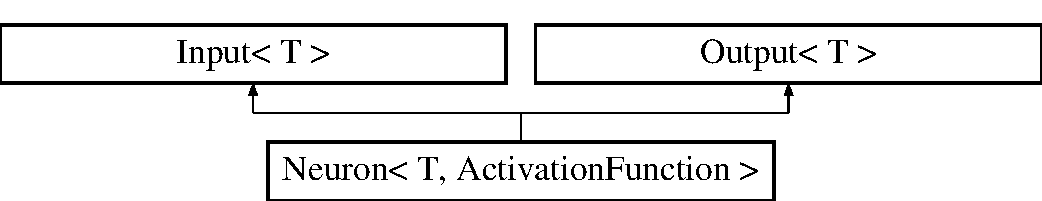
\includegraphics[height=2.000000cm]{class_neuron}
\end{center}
\end{figure}
\subsection*{\-Public \-Member \-Functions}
\begin{DoxyCompactItemize}
\item 
\hyperlink{class_neuron_ada8bb503f1bd56ce2596eabf8c21877e}{\-Neuron} ()
\item 
\hyperlink{class_neuron_a6145b98854c0fb6e9cfe09336952a5dc}{\-Neuron} (\-T lf)
\item 
\hyperlink{class_neuron_afff69f38459625c7d376e5f5e2e34a9d}{\-Neuron} (\hyperlink{class_activation_function}{\-Activation\-Function} fun)
\item 
\hyperlink{class_neuron_a1c7ea1b973546b185e6ec0c29b740453}{\-Neuron} (\hyperlink{class_activation_function}{\-Activation\-Function} fun, \-T lf)
\item 
void \hyperlink{class_neuron_a36c60982cb604f2fa6a1765177a9c2e7}{calculate\-Output} ()
\item 
void \hyperlink{class_neuron_ae73a056c55311521d0e31347837109cc}{learn\-Delta} ()
\item 
void \hyperlink{class_neuron_acb55ff03a770877b6afb86ed4d06896a}{propagate\-Answer} ()
\item 
void \hyperlink{class_neuron_a5e479fce295d76be68c017ab8c986f8c}{learn\-B\-P} ()
\item 
\hypertarget{class_neuron_a7ab012ac0a6a20b474b6147fcdc6ea2d}{void {\bfseries check\-Wages} ()}\label{class_neuron_a7ab012ac0a6a20b474b6147fcdc6ea2d}

\item 
void \hyperlink{class_neuron_a1a20d9ac9bf64126f8d74d8c1c7d3c58}{set\-Link\-In} (\hyperlink{class_link}{\-Link}$<$ \-T $>$ $\ast$link)
\end{DoxyCompactItemize}


\subsection{\-Detailed \-Description}
\subsubsection*{template$<$class T, class Activation\-Function = \-Step\-Activation\-Function$<$\-T$>$()$>$class Neuron$<$ T, Activation\-Function $>$}

\-Klasa \hyperlink{class_neuron}{\-Neuron} odpowiada neuronowi w sieci neuronowej. \-Podana funkcja aktywacji jest klasą zawierającą metody\-: operator() za pomocą, której jest wyliczane pobudzenie neuronu oraz deriterative(\-T x) pozwalającą na wyznaczenie pochodnej funkcji aktywacji w punkcie x (jest to niezbędne do realizacji procesu uczenia się sieci). \-Współczynnik uczenia jest ustalony na sztywno na 0.\-7 (co z tym idzie aby sieć mogła się uczyć nie należy używać liczb całkowytych). 

\subsection{\-Constructor \& \-Destructor \-Documentation}
\hypertarget{class_neuron_ada8bb503f1bd56ce2596eabf8c21877e}{\index{\-Neuron@{\-Neuron}!\-Neuron@{\-Neuron}}
\index{\-Neuron@{\-Neuron}!Neuron@{\-Neuron}}
\subsubsection[{\-Neuron}]{\setlength{\rightskip}{0pt plus 5cm}template$<$class T , class Activation\-Function  = \-Step\-Activation\-Function$<$\-T$>$()$>$ {\bf \-Neuron}$<$ \-T, {\bf \-Activation\-Function} $>$\-::{\bf \-Neuron} (
\begin{DoxyParamCaption}
{}
\end{DoxyParamCaption}
)\hspace{0.3cm}{\ttfamily  \mbox{[}inline\mbox{]}}}}\label{class_neuron_ada8bb503f1bd56ce2596eabf8c21877e}
\-Konstruktor domyślny z ustawieniem współczynnika uczenia z funkcją aktywacji, która jest funkcją skokową i skoku w punkcie 0. \-Współczynnik uczenie ustawiony jest na 0.\-7. 
\begin{DoxyParams}{\-Parameters}
{\em lf} & \-Współczynnik uczenia. \\
\hline
\end{DoxyParams}
\hypertarget{class_neuron_a6145b98854c0fb6e9cfe09336952a5dc}{\index{\-Neuron@{\-Neuron}!\-Neuron@{\-Neuron}}
\index{\-Neuron@{\-Neuron}!Neuron@{\-Neuron}}
\subsubsection[{\-Neuron}]{\setlength{\rightskip}{0pt plus 5cm}template$<$class T , class Activation\-Function  = \-Step\-Activation\-Function$<$\-T$>$()$>$ {\bf \-Neuron}$<$ \-T, {\bf \-Activation\-Function} $>$\-::{\bf \-Neuron} (
\begin{DoxyParamCaption}
\item[{\-T}]{lf}
\end{DoxyParamCaption}
)\hspace{0.3cm}{\ttfamily  \mbox{[}inline\mbox{]}}}}\label{class_neuron_a6145b98854c0fb6e9cfe09336952a5dc}
\-Konstruktor parametryczny z ustawieniem współczynnika uczenia oraz z funkcją aktywacji, która jest funkcją skokową i skoku w punkcie 0. 
\begin{DoxyParams}{\-Parameters}
{\em lf} & \-Współczynnik uczenia. \\
\hline
\end{DoxyParams}
\hypertarget{class_neuron_afff69f38459625c7d376e5f5e2e34a9d}{\index{\-Neuron@{\-Neuron}!\-Neuron@{\-Neuron}}
\index{\-Neuron@{\-Neuron}!Neuron@{\-Neuron}}
\subsubsection[{\-Neuron}]{\setlength{\rightskip}{0pt plus 5cm}template$<$class T , class Activation\-Function  = \-Step\-Activation\-Function$<$\-T$>$()$>$ {\bf \-Neuron}$<$ \-T, {\bf \-Activation\-Function} $>$\-::{\bf \-Neuron} (
\begin{DoxyParamCaption}
\item[{{\bf \-Activation\-Function}}]{fun}
\end{DoxyParamCaption}
)\hspace{0.3cm}{\ttfamily  \mbox{[}inline\mbox{]}}}}\label{class_neuron_afff69f38459625c7d376e5f5e2e34a9d}
\-Konstruktor parametryczny z ustawieniem funkcji aktywacji. \-Jako współczynnik uczenia ustawione jest 0.\-7. 
\begin{DoxyParams}{\-Parameters}
{\em fun} & \-Funkcja aktywacji. \\
\hline
\end{DoxyParams}
\hypertarget{class_neuron_a1c7ea1b973546b185e6ec0c29b740453}{\index{\-Neuron@{\-Neuron}!\-Neuron@{\-Neuron}}
\index{\-Neuron@{\-Neuron}!Neuron@{\-Neuron}}
\subsubsection[{\-Neuron}]{\setlength{\rightskip}{0pt plus 5cm}template$<$class T , class Activation\-Function  = \-Step\-Activation\-Function$<$\-T$>$()$>$ {\bf \-Neuron}$<$ \-T, {\bf \-Activation\-Function} $>$\-::{\bf \-Neuron} (
\begin{DoxyParamCaption}
\item[{{\bf \-Activation\-Function}}]{fun, }
\item[{\-T}]{lf}
\end{DoxyParamCaption}
)\hspace{0.3cm}{\ttfamily  \mbox{[}inline\mbox{]}}}}\label{class_neuron_a1c7ea1b973546b185e6ec0c29b740453}
\-Konstruktor parametryczny z ustawieniem funkcji aktywacji i współczynnika uczenia. 
\begin{DoxyParams}{\-Parameters}
{\em fun} & \-Funkcja aktywacji. \\
\hline
{\em lf} & \-Współczynnik uczenia. \\
\hline
\end{DoxyParams}


\subsection{\-Member \-Function \-Documentation}
\hypertarget{class_neuron_a36c60982cb604f2fa6a1765177a9c2e7}{\index{\-Neuron@{\-Neuron}!calculate\-Output@{calculate\-Output}}
\index{calculate\-Output@{calculate\-Output}!Neuron@{\-Neuron}}
\subsubsection[{calculate\-Output}]{\setlength{\rightskip}{0pt plus 5cm}template$<$class T , class Activation\-Function  = \-Step\-Activation\-Function$<$\-T$>$()$>$ void {\bf \-Neuron}$<$ \-T, {\bf \-Activation\-Function} $>$\-::{\bf calculate\-Output} (
\begin{DoxyParamCaption}
{}
\end{DoxyParamCaption}
)\hspace{0.3cm}{\ttfamily  \mbox{[}inline\mbox{]}}}}\label{class_neuron_a36c60982cb604f2fa6a1765177a9c2e7}
\-Funkcja licząca wyjście neuronu w zależności od wejsć (suma ważone) a następnie przejście przez funkcję aktywacji. \hypertarget{class_neuron_a5e479fce295d76be68c017ab8c986f8c}{\index{\-Neuron@{\-Neuron}!learn\-B\-P@{learn\-B\-P}}
\index{learn\-B\-P@{learn\-B\-P}!Neuron@{\-Neuron}}
\subsubsection[{learn\-B\-P}]{\setlength{\rightskip}{0pt plus 5cm}template$<$class T , class Activation\-Function  = \-Step\-Activation\-Function$<$\-T$>$()$>$ void {\bf \-Neuron}$<$ \-T, {\bf \-Activation\-Function} $>$\-::{\bf learn\-B\-P} (
\begin{DoxyParamCaption}
{}
\end{DoxyParamCaption}
)\hspace{0.3cm}{\ttfamily  \mbox{[}inline\mbox{]}}}}\label{class_neuron_a5e479fce295d76be68c017ab8c986f8c}
\-Funkcja ucząca wg reguły \-Back \-Propagation dla warstw ukrytych. \hypertarget{class_neuron_ae73a056c55311521d0e31347837109cc}{\index{\-Neuron@{\-Neuron}!learn\-Delta@{learn\-Delta}}
\index{learn\-Delta@{learn\-Delta}!Neuron@{\-Neuron}}
\subsubsection[{learn\-Delta}]{\setlength{\rightskip}{0pt plus 5cm}template$<$class T , class Activation\-Function  = \-Step\-Activation\-Function$<$\-T$>$()$>$ void {\bf \-Neuron}$<$ \-T, {\bf \-Activation\-Function} $>$\-::{\bf learn\-Delta} (
\begin{DoxyParamCaption}
{}
\end{DoxyParamCaption}
)\hspace{0.3cm}{\ttfamily  \mbox{[}inline\mbox{]}}}}\label{class_neuron_ae73a056c55311521d0e31347837109cc}
\-Funkcja ucząca wg reguły delta. \-Stosowana tylko dla sieci jednowarstwowych. 
\begin{DoxyParams}{\-Parameters}
{\em answer} & \-Wymagana odpowiedź dla danego neuronu. \\
\hline
\end{DoxyParams}
\hypertarget{class_neuron_acb55ff03a770877b6afb86ed4d06896a}{\index{\-Neuron@{\-Neuron}!propagate\-Answer@{propagate\-Answer}}
\index{propagate\-Answer@{propagate\-Answer}!Neuron@{\-Neuron}}
\subsubsection[{propagate\-Answer}]{\setlength{\rightskip}{0pt plus 5cm}template$<$class T , class Activation\-Function  = \-Step\-Activation\-Function$<$\-T$>$()$>$ void {\bf \-Neuron}$<$ \-T, {\bf \-Activation\-Function} $>$\-::{\bf propagate\-Answer} (
\begin{DoxyParamCaption}
{}
\end{DoxyParamCaption}
)\hspace{0.3cm}{\ttfamily  \mbox{[}inline\mbox{]}}}}\label{class_neuron_acb55ff03a770877b6afb86ed4d06896a}
\-Funkcja propagująca błąd do głębszych warstw sieci. \hypertarget{class_neuron_a1a20d9ac9bf64126f8d74d8c1c7d3c58}{\index{\-Neuron@{\-Neuron}!set\-Link\-In@{set\-Link\-In}}
\index{set\-Link\-In@{set\-Link\-In}!Neuron@{\-Neuron}}
\subsubsection[{set\-Link\-In}]{\setlength{\rightskip}{0pt plus 5cm}template$<$class T , class Activation\-Function  = \-Step\-Activation\-Function$<$\-T$>$()$>$ void {\bf \-Neuron}$<$ \-T, {\bf \-Activation\-Function} $>$\-::{\bf set\-Link\-In} (
\begin{DoxyParamCaption}
\item[{{\bf \-Link}$<$ \-T $>$ $\ast$}]{link}
\end{DoxyParamCaption}
)\hspace{0.3cm}{\ttfamily  \mbox{[}inline\mbox{]}}}}\label{class_neuron_a1a20d9ac9bf64126f8d74d8c1c7d3c58}
\-Funkcja ustawiająca połączenie wejściowe oraz dodające nową wagę. 
\begin{DoxyParams}{\-Parameters}
{\em link} & \-Połączenie do ododania. \\
\hline
\end{DoxyParams}


\-Reimplemented from \hyperlink{class_output_afd26f81d178846371c17d63015f2eb9f}{\-Output$<$ T $>$}.



\-The documentation for this class was generated from the following file\-:\begin{DoxyCompactItemize}
\item 
\-Neuron/\-Neuron.\-h\end{DoxyCompactItemize}

\hypertarget{class_output}{\section{\-Output$<$ \-T $>$ \-Class \-Template \-Reference}
\label{class_output}\index{\-Output$<$ T $>$@{\-Output$<$ T $>$}}
}


{\ttfamily \#include $<$\-Output.\-h$>$}

\-Inheritance diagram for \-Output$<$ \-T $>$\-:\begin{figure}[H]
\begin{center}
\leavevmode
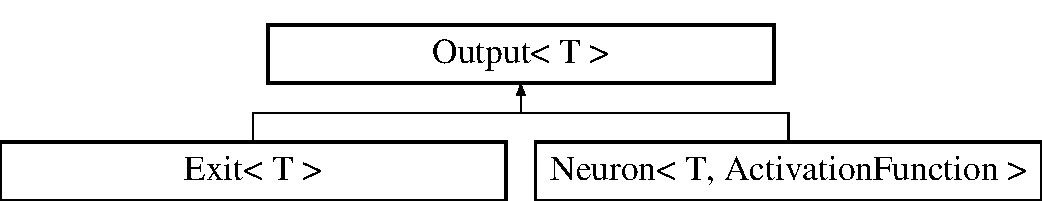
\includegraphics[height=2.000000cm]{class_output}
\end{center}
\end{figure}
\subsection*{\-Public \-Member \-Functions}
\begin{DoxyCompactItemize}
\item 
virtual \hyperlink{class_output_aebe365bb0c9844b5456e74f0fb1a0a35}{$\sim$\-Output} ()
\item 
void \hyperlink{class_output_afd26f81d178846371c17d63015f2eb9f}{set\-Link\-In} (\hyperlink{class_link}{\-Link}$<$ \-T $>$ $\ast$link)
\end{DoxyCompactItemize}
\subsection*{\-Protected \-Attributes}
\begin{DoxyCompactItemize}
\item 
\hypertarget{class_output_ade68e41659b12f8a7e31f8dc8507bb50}{std\-::list$<$ \hyperlink{class_link}{\-Link}$<$ \-T $>$ $\ast$ $>$ {\bfseries ins}}\label{class_output_ade68e41659b12f8a7e31f8dc8507bb50}

\end{DoxyCompactItemize}


\subsection{\-Detailed \-Description}
\subsubsection*{template$<$class \-T$>$class Output$<$ T $>$}

\-Klasa \hyperlink{class_output}{\-Output} jest interfejsem wyjścia dla klasy \hyperlink{class_link}{\-Link}. 

\subsection{\-Constructor \& \-Destructor \-Documentation}
\hypertarget{class_output_aebe365bb0c9844b5456e74f0fb1a0a35}{\index{\-Output@{\-Output}!$\sim$\-Output@{$\sim$\-Output}}
\index{$\sim$\-Output@{$\sim$\-Output}!Output@{\-Output}}
\subsubsection[{$\sim$\-Output}]{\setlength{\rightskip}{0pt plus 5cm}template$<$class \-T$>$ virtual {\bf \-Output}$<$ \-T $>$\-::$\sim${\bf \-Output} (
\begin{DoxyParamCaption}
{}
\end{DoxyParamCaption}
)\hspace{0.3cm}{\ttfamily  \mbox{[}inline, virtual\mbox{]}}}}\label{class_output_aebe365bb0c9844b5456e74f0fb1a0a35}
\-Destruktor. 

\subsection{\-Member \-Function \-Documentation}
\hypertarget{class_output_afd26f81d178846371c17d63015f2eb9f}{\index{\-Output@{\-Output}!set\-Link\-In@{set\-Link\-In}}
\index{set\-Link\-In@{set\-Link\-In}!Output@{\-Output}}
\subsubsection[{set\-Link\-In}]{\setlength{\rightskip}{0pt plus 5cm}template$<$class \-T$>$ void {\bf \-Output}$<$ \-T $>$\-::{\bf set\-Link\-In} (
\begin{DoxyParamCaption}
\item[{{\bf \-Link}$<$ \-T $>$ $\ast$}]{link}
\end{DoxyParamCaption}
)\hspace{0.3cm}{\ttfamily  \mbox{[}inline\mbox{]}}}}\label{class_output_afd26f81d178846371c17d63015f2eb9f}
\-Funkcja przyjmująca wartość z łącza. 
\begin{DoxyParams}{\-Parameters}
{\em o} & \-Otrzymana wartość z łącza. \-Funkcja dodająca połączenie do wyjścia z połączenia. \\
\hline
{\em link} & \-Dodawane połączenie. \\
\hline
\end{DoxyParams}


\-Reimplemented in \hyperlink{class_neuron_a1a20d9ac9bf64126f8d74d8c1c7d3c58}{\-Neuron$<$ T, Activation\-Function $>$}.



\-The documentation for this class was generated from the following file\-:\begin{DoxyCompactItemize}
\item 
\-Neuron/\-Output.\-h\end{DoxyCompactItemize}

\hypertarget{class_step_activation_function}{\section{\-Step\-Activation\-Function$<$ \-T $>$ \-Class \-Template \-Reference}
\label{class_step_activation_function}\index{\-Step\-Activation\-Function$<$ T $>$@{\-Step\-Activation\-Function$<$ T $>$}}
}


{\ttfamily \#include $<$\-Step\-Activation\-Function.\-h$>$}

\subsection*{\-Public \-Member \-Functions}
\begin{DoxyCompactItemize}
\item 
\hyperlink{class_step_activation_function_abcd92f0d83e917f9e7bc57caadf8af45}{\-Step\-Activation\-Function} ()
\item 
\hyperlink{class_step_activation_function_ac28ff4d93eb28f878b174630d4023c67}{\-Step\-Activation\-Function} (\-T i)
\item 
\-T \hyperlink{class_step_activation_function_a2b243dae27dd2ba5458acc5a32d4c542}{operator()} (\-T x)
\item 
\-T \hyperlink{class_step_activation_function_ad85d33127de89670f9c8a46ec1d5dd55}{deriterative} (\-T x)
\end{DoxyCompactItemize}


\subsection{\-Detailed \-Description}
\subsubsection*{template$<$class T$>$class Step\-Activation\-Function$<$ T $>$}

\-Klasa przedstawiającą skokową funkcję aktywacji o określonym progu. \-Aktywacja następuje gdy dana wartość jest większa od wartości progu. \-Pochodną funkcji jest zookrąglona delta diraca. 

\subsection{\-Constructor \& \-Destructor \-Documentation}
\hypertarget{class_step_activation_function_abcd92f0d83e917f9e7bc57caadf8af45}{\index{\-Step\-Activation\-Function@{\-Step\-Activation\-Function}!\-Step\-Activation\-Function@{\-Step\-Activation\-Function}}
\index{\-Step\-Activation\-Function@{\-Step\-Activation\-Function}!StepActivationFunction@{\-Step\-Activation\-Function}}
\subsubsection[{\-Step\-Activation\-Function}]{\setlength{\rightskip}{0pt plus 5cm}template$<$class T $>$ {\bf \-Step\-Activation\-Function}$<$ \-T $>$\-::{\bf \-Step\-Activation\-Function} (
\begin{DoxyParamCaption}
{}
\end{DoxyParamCaption}
)\hspace{0.3cm}{\ttfamily  \mbox{[}inline\mbox{]}}}}\label{class_step_activation_function_abcd92f0d83e917f9e7bc57caadf8af45}
\-Konstrutor domyślny ustawiający za wartość 0 (rzutowaną na dany typ) \hypertarget{class_step_activation_function_ac28ff4d93eb28f878b174630d4023c67}{\index{\-Step\-Activation\-Function@{\-Step\-Activation\-Function}!\-Step\-Activation\-Function@{\-Step\-Activation\-Function}}
\index{\-Step\-Activation\-Function@{\-Step\-Activation\-Function}!StepActivationFunction@{\-Step\-Activation\-Function}}
\subsubsection[{\-Step\-Activation\-Function}]{\setlength{\rightskip}{0pt plus 5cm}template$<$class T $>$ {\bf \-Step\-Activation\-Function}$<$ \-T $>$\-::{\bf \-Step\-Activation\-Function} (
\begin{DoxyParamCaption}
\item[{\-T}]{i}
\end{DoxyParamCaption}
)\hspace{0.3cm}{\ttfamily  \mbox{[}inline\mbox{]}}}}\label{class_step_activation_function_ac28ff4d93eb28f878b174630d4023c67}
\-Konstruktor z parametrem progu. 
\begin{DoxyParams}{\-Parameters}
{\em i} & \-Próg jaki chcemy ustawić. \\
\hline
\end{DoxyParams}


\subsection{\-Member \-Function \-Documentation}
\hypertarget{class_step_activation_function_ad85d33127de89670f9c8a46ec1d5dd55}{\index{\-Step\-Activation\-Function@{\-Step\-Activation\-Function}!deriterative@{deriterative}}
\index{deriterative@{deriterative}!StepActivationFunction@{\-Step\-Activation\-Function}}
\subsubsection[{deriterative}]{\setlength{\rightskip}{0pt plus 5cm}template$<$class T $>$ \-T {\bf \-Step\-Activation\-Function}$<$ \-T $>$\-::{\bf deriterative} (
\begin{DoxyParamCaption}
\item[{\-T}]{x}
\end{DoxyParamCaption}
)\hspace{0.3cm}{\ttfamily  \mbox{[}inline\mbox{]}}}}\label{class_step_activation_function_ad85d33127de89670f9c8a46ec1d5dd55}
\-Funkcja licząca pochodną funkcji skokowej (jako cos(x) w zakresie 0 do 1) 
\begin{DoxyParams}{\-Parameters}
{\em x} & \\
\hline
\end{DoxyParams}
\begin{DoxyReturn}{\-Returns}

\end{DoxyReturn}
\hypertarget{class_step_activation_function_a2b243dae27dd2ba5458acc5a32d4c542}{\index{\-Step\-Activation\-Function@{\-Step\-Activation\-Function}!operator()@{operator()}}
\index{operator()@{operator()}!StepActivationFunction@{\-Step\-Activation\-Function}}
\subsubsection[{operator()}]{\setlength{\rightskip}{0pt plus 5cm}template$<$class T $>$ \-T {\bf \-Step\-Activation\-Function}$<$ \-T $>$\-::operator() (
\begin{DoxyParamCaption}
\item[{\-T}]{x}
\end{DoxyParamCaption}
)\hspace{0.3cm}{\ttfamily  \mbox{[}inline\mbox{]}}}}\label{class_step_activation_function_a2b243dae27dd2ba5458acc5a32d4c542}
\-Funkcja sprawdzająca czy dana wartość jest większa od podanego progu. 
\begin{DoxyParams}{\-Parameters}
{\em x} & \-Sprawdzana wartość. \\
\hline
\end{DoxyParams}
\begin{DoxyReturn}{\-Returns}
1 jeśli sprawdzana waratość jest większa, 0 w przeciwnym wypadku. 
\end{DoxyReturn}


\-The documentation for this class was generated from the following file\-:\begin{DoxyCompactItemize}
\item 
\-Neuron/\-Step\-Activation\-Function.\-h\end{DoxyCompactItemize}

\hypertarget{class_neural_network_1_1_wrong_argument}{\section{\-Neural\-Network$<$ \-T, \-Activation\-Function $>$\-:\-:\-Wrong\-Argument \-Class \-Reference}
\label{class_neural_network_1_1_wrong_argument}\index{\-Neural\-Network$<$ T, Activation\-Function $>$\-::\-Wrong\-Argument@{\-Neural\-Network$<$ T, Activation\-Function $>$\-::\-Wrong\-Argument}}
}
\subsection*{\-Public \-Member \-Functions}
\begin{DoxyCompactItemize}
\item 
\hypertarget{class_neural_network_1_1_wrong_argument_a7dddcaf96b854ada5554b05e0429ea6a}{{\bfseries \-Wrong\-Argument} (std\-::string m)}\label{class_neural_network_1_1_wrong_argument_a7dddcaf96b854ada5554b05e0429ea6a}

\item 
\hypertarget{class_neural_network_1_1_wrong_argument_a708ad656cec99bc65e351dec562c5402}{std\-::string {\bfseries \-Get\-Message} () const }\label{class_neural_network_1_1_wrong_argument_a708ad656cec99bc65e351dec562c5402}

\end{DoxyCompactItemize}
\subsubsection*{template$<$class T, class Activation\-Function$>$ class Neural\-Network$<$ T, Activation\-Function $>$\-::\-Wrong\-Argument}



\-The documentation for this class was generated from the following file\-:\begin{DoxyCompactItemize}
\item 
\-Neural\-Network/\-Neural\-Network.\-h\end{DoxyCompactItemize}

\hypertarget{class_neural_network_1_1_wrong_state}{\section{\-Neural\-Network$<$ \-T, \-Activation\-Function $>$\-:\-:\-Wrong\-State \-Class \-Reference}
\label{class_neural_network_1_1_wrong_state}\index{\-Neural\-Network$<$ T, Activation\-Function $>$\-::\-Wrong\-State@{\-Neural\-Network$<$ T, Activation\-Function $>$\-::\-Wrong\-State}}
}
\subsubsection*{template$<$class T, class Activation\-Function$>$ class Neural\-Network$<$ T, Activation\-Function $>$\-::\-Wrong\-State}



\-The documentation for this class was generated from the following file\-:\begin{DoxyCompactItemize}
\item 
\-Neural\-Network/\-Neural\-Network.\-h\end{DoxyCompactItemize}

\printindex
\end{document}
